\documentclass[sigconf,authordraft,natbib=false]{acmart}

\usepackage{graphicx}
\usepackage[utf8]{inputenc}
\usepackage{blindtext}
\usepackage{listings}
\usepackage{attachfile}
\usepackage{cleveref}
\usepackage{fontawesome}
\usepackage{csquotes}
\usepackage{subcaption}
\usepackage{float}
\usepackage[hyphens]{xurl}

\acmConference[FWS2026]{Abschlusskonferenz FWS/SDUT Sommersemester 2026}{July 01, 2026}{Ingolstadt, DE}

\RequirePackage[
  datamodel=acmdatamodel,
  style=acmauthoryear,
  ]{biblatex}

\addbibresource{ai-automation-bias.bib}

\title[AI Fallibility \& Automation Bias long-term Effects]{The Long-Term Effects of Indicating AI Fallibility on Automation Bias in Mental Health Application Users}

\author{Tim Ruland}
\authornote{These authors contributed equally to this in research, organization, writing and everything else.}


\author{Marc Obst}
\authornotemark[1]

\author{Nicolas Weber}
\authornotemark[1]
\affiliation{
  \institution{Technische Hochschule Ingolstadt}
  \city{Ingolstadt}
  \country{Germany}}

\author{Emely Rosbach}
\affiliation{
  \institution{Technische Hochschule Ingolstadt}
  \city{Ingolstadt}
  \country{Germany}}
\email{emr@thi.de}

\renewcommand{\shortauthors}{Gerhardinger et al.}

\usepackage[acronym]{glossaries}


\makeglossaries

% -------------------------
% Acronyms
% -------------------------

\newacronym{abs}{\(B\)}{Automation Bias Score}
\newacronym{mean-abs}{\(\bar{B}\)}{Mean Automation Bias Score}
\newacronym{h1}{\(H_1\)}{Hypothesis 1: Short Term Effect}
\newacronym{h2}{\(H_2\)}{Hypothesis 2: Long Term Effect}
\newacronym{G}{\(G\)}{possible participant groups}
\newacronym{C}{\(C\)}{possible case vignettes}
\newacronym{T}{\(T\)}{possible truth values}
\newacronym{R}{\(R\)}{possible rounds for participants}
\newacronym{S}{\(S\)}{possible sessions for participants}
\newacronym{S2}{\(S^2\)}{possible session combinations for participants}
\newacronym{P}{\(P\)}{possible participants}

\newacronym{ai}{AI}{Artificial Intelligence}
\newacronym{ueq-plus}{UEQ+}{User Experience Questionnaire Plus}
\newacronym{thi}{THI}{Technische Hochschule Ingolstadt}
\newacronym[
    description={A web application that uses modern web technologies to provide an app-like experience, including offline functionality, responsiveness, and installability across different devices and platforms}
]{pwa}{PWA}{Progressive Web App}

% -------------------------
% Glossary Entries
% -------------------------


\newglossaryentry{pseudo-random-seed}
{
name=pseudo-random seed,
plural=pseudo-random seeds,
description={A fixed numerical value used to ensure reproducibility of pseudo-random participant allocation}
}



\begin{document}

\hypersetup{
    hidelinks,
    breaklinks=true
}


\Urlmuskip=0mu plus 1mu\relax

\begin{abstract}
This study examined the short and long-term effects of disclaimer messages on participants’ evaluations of \gls{ai}-generated mental health recommendations, focusing on automation bias.
A mixed longitudinal design with two sessions, separated by one week, was used.
Participants first completed a questionnaire on their attitudes toward AI, reviewed a mental health case vignette, and requested an \gls{ai}-based assessment. After evaluating the generated recommendation, they completed a post-interaction questionnaire.
Participants in the active group received two disclaimers during Session 1: a full-screen disclaimer and an inline disclaimer.
Results indicate that disclaimers may reduce automation bias initially, but this effect did not persist over time. In Session 2, a rebound effect emerged, with the active group showing higher automation bias scores.
In contrast, the control group displayed lower automation bias in Session 2 compared to Session 1, suggesting a shift toward more critical evaluation of \gls{ai}-generated recommendations.
\end{abstract}

%%
%% The code below is generated by the tool at http://dl.acm.org/ccs.cfm.
%% DO NOT CHANGE MANUALLY
%%
\begin{CCSXML}
<ccs2012>
   <concept>
       <concept_id>10002951.10003317.10003331</concept_id>
       <concept_desc>Information systems~Users and interactive retrieval</concept_desc>
       <concept_significance>500</concept_significance>
       </concept>
   <concept>
       <concept_id>10002951.10003317.10003359</concept_id>
       <concept_desc>Information systems~Evaluation of retrieval results</concept_desc>
       <concept_significance>500</concept_significance>
       </concept>
   <concept>
       <concept_id>10002944.10011122.10002945</concept_id>
       <concept_desc>General and reference~Surveys and overviews</concept_desc>
       <concept_significance>500</concept_significance>
       </concept>
   <concept>
       <concept_id>10010147.10010178.10010187</concept_id>
       <concept_desc>Computing methodologies~Knowledge representation and reasoning</concept_desc>
       <concept_significance>100</concept_significance>
       </concept>
   <concept>
       <concept_id>10010147.10010178</concept_id>
       <concept_desc>Computing methodologies~Artificial intelligence</concept_desc>
       <concept_significance>500</concept_significance>
       </concept>
   <concept>
       <concept_id>10003456.10010927.10010930</concept_id>
       <concept_desc>Social and professional topics~Age</concept_desc>
       <concept_significance>100</concept_significance>
       </concept>
   <concept>
       <concept_id>10003456.10010927.10003613</concept_id>
       <concept_desc>Social and professional topics~Gender</concept_desc>
       <concept_significance>100</concept_significance>
       </concept>
   <concept>
       <concept_id>10003120.10003121</concept_id>
       <concept_desc>Human-centered computing~Human computer interaction (HCI)</concept_desc>
       <concept_significance>100</concept_significance>
       </concept>
   <concept>
       <concept_id>10003120.10003123.10011759</concept_id>
       <concept_desc>Human-centered computing~Empirical studies in interaction design</concept_desc>
       <concept_significance>500</concept_significance>
       </concept>
   <concept>
       <concept_id>10003120.10003145</concept_id>
       <concept_desc>Human-centered computing~Visualization</concept_desc>
       <concept_significance>300</concept_significance>
       </concept>
   <concept>
       <concept_id>10003120.10003121.10011748</concept_id>
       <concept_desc>Human-centered computing~Empirical studies in HCI</concept_desc>
       <concept_significance>500</concept_significance>
       </concept>
 </ccs2012>
\end{CCSXML}

\ccsdesc[500]{Information systems~Users and interactive retrieval}
\ccsdesc[500]{Information systems~Evaluation of retrieval results}
\ccsdesc[500]{General and reference~Surveys and overviews}
\ccsdesc[100]{Computing methodologies~Knowledge representation and reasoning}
\ccsdesc[500]{Computing methodologies~Artificial intelligence}
\ccsdesc[100]{Social and professional topics~Age}
\ccsdesc[100]{Social and professional topics~Gender}
\ccsdesc[100]{Human-centered computing~Human computer interaction (HCI)}
\ccsdesc[500]{Human-centered computing~Empirical studies in interaction design}
\ccsdesc[300]{Human-centered computing~Visualization}
\ccsdesc[500]{Human-centered computing~Empirical studies in HCI}


\keywords{Mental Health, AI, Artificial Intelligence, FWS, STUD, automation bias, Fallibility, Mental Health Application, \Gls{ai} Assistant, Long-Term, Long-Term Effects, Priming, Trust, Confidence}

\maketitle


\section{Introduction}
Mental health remains one of the most prevalent yet underrepresented topics in society.
Although awareness of mental health issues has increased in recent years, many challenges regarding access to adequate support and treatment persist.
These issues became particularly apparent during the COVID-19 pandemic in 2020 and the years that followed, when a significant decline in adult mental well-being was observed worldwide \autocite[]{robert_koch_public_health_reporting}.
The increased prevalence of psychological distress, combined with limited availability of professional mental health services, has highlighted the need for scalable and accessible forms of support.

At the same time, \Gls{ai} has rapidly been integrated into a wide range of domains, including healthcare and, more specifically, mental health care.
In this context, \Gls{ai} offers considerable potential to complement existing services by enabling early detection of mental health conditions, providing personalized treatment recommendations, and helping to prevent the escalation of symptoms \autocite[]{mikaeili_reimagining_2025}.
Furthermore, machine learning algorithms have already demonstrated promising performance in classifying mental disorders and predicting treatment responses, indicating that \Gls{ai} could become a valuable tool for supporting both patients and healthcare professionals \autocite[]{gonzalez_systematic_review}.
As AI-based applications become increasingly accessible to the general public, they may also help alleviate some of the pressure on already overburdened healthcare systems. Machine learning algorithms already show efficacy in classifying mental disorders and treatment responses, which suggests a promising potential \autocite[]{gonzalez_systematic_review}.

Despite these opportunities, the growing integration of \Gls{ai} into mental health care raises several important concerns.
Issues related to accessibility, data privacy and security, cultural diversity, and fairness remain critical challenges that need to be addressed \autocite[]{ali_artificial_2025}.
In particular, algorithmic biases have received increasing attention, as biased systems may produce inaccurate or potentially harmful recommendations for certain user groups.
However, focusing solely on algorithmic bias neglects another important aspect: the role of the human user.
Individuals interacting with \Gls{ai} systems may themselves be susceptible to cognitive biases that influence their decision-making processes.

One such phenomenon is automation bias, which describes the tendency of users to over-rely on automated systems and accept their recommendations without sufficient critical evaluation \autocite[p~391]{parasuraman_complacency_2010}. 
In the context of mental health, this issue is especially relevant, as decisions based on AI-generated advice may have substantial consequences for an individual’s well-being.
Therefore, the human factor should not be overlooked when evaluating the safe and responsible implementation of \Gls{ai} in mental health applications. 

To address this research gap, the present study investigates human automation bias in the use of \Gls{ai} for mental health support.
More specifically, we examine whether the inclusion of disclaimers can influence users’ interactions with AI-generated recommendations and encourage a more critical evaluation of the provided information.
Previous research by \citeauthor*[]{wingerter_mitigating_2025} showed that warning nudges communicating the fallibility of \Gls{ai} can mitigate automation bias to a certain extent \autocite[]{wingerter_mitigating_2025}.
However, these findings were obtained in a different application context and cannot necessarily be generalized to mental health scenarios.
Given the sensitivity and potential risks associated with mental health support, it is essential to investigate whether similar interventions are effective in this domain.
Consequently, this study examines the impact of warning nudges—in the form of disclaimers—on users’ reliance on \Gls{ai} within a mental health context. These disclaimers will be integrated into a PWA which we will design specifically for this study. 


\section{Related Work}
\Gls{ai} is increasingly being integrated into mental health care, where it is used for diagnostic support, therapy assistance, behavioral monitoring, and clinical decision-making.
\citeauthor[]{ali_artificial_2025} provide a comprehensive overview of current \Gls{ai} applications in mental health and highlight the potential of machine learning, deep learning, and natural language processing to improve accessibility, personalization, and early detection of mental health conditions.
In particular, AI-powered chatbots and recommendation systems have emerged as scalable tools capable of delivering therapeutic support and psychoeducation.
At the same time, the authors emphasize several challenges, including privacy concerns, algorithmic bias, transparency, and the risk of over-reliance on automated recommendations.
They conclude that successful deployment of \Gls{ai} in mental health requires not only technical accuracy but also responsible human-AI interaction and appropriate safeguards against misuse \autocite[]{ali_artificial_2025}.

Automation bias describes the tendency of users to place excessive trust in automated recommendations and insufficiently verify their correctness \autocite[p~391]{parasuraman_complacency_2010}.
In recent times, this phenomenon has been increasingly observed to occur in interactions with generative \Gls{ai} systems \autocite[]{kucking_automation_2026}.
\citeauthor[]{wingerter_mitigating_2025} investigated this effect using a Cognitive Reflection Test (CRT) in which participants received deliberately incorrect AI-generated recommendations.
Their results demonstrated that participants exposed to faulty \Gls{ai} advice performed significantly worse than participants without \Gls{ai} support, indicating a substantial automation bias effect \autocite[]{wingerter_mitigating_2025}.

To mitigate this effect, \citeauthor[]{wingerter_mitigating_2025} introduced a warning nudge reminding users that \gls{ai}-generated outputs may be inaccurate or biased.
Participants who received this warning achieved substantially better performance than participants who received incorrect \gls{ai} advice without a warning.
The warning nearly doubled performance relative to the faulty-\gls{ai} condition and reduced automation bias to a level comparable to the control group.
Interestingly, self-reported \Gls{ai} literacy did not significantly reduce susceptibility to automation bias, suggesting that interface design interventions may be more effective than user experience or prior \Gls{ai} knowledge alone.


While \citeauthor[]{wingerter_mitigating_2025} demonstrate that warning nudges can reduce automation bias during a single interaction with generative AI, their study does not investigate whether such effects persist over time.
Furthermore, their experiment was conducted using abstract cognitive-reflection tasks rather than domain-specific scenarios.
\autocite[]{wingerter_mitigating_2025}
At the same time, recent reviews of \Gls{ai} in mental health emphasize that user trust, transparency, and human-AI interaction are critical factors for the successful adoption of AI-supported mental health applications, while long-term behavioral effects remain largely unexplored \autocite[]{mikaeili_reimagining_2025}.

In contrast, the present study examines the influence of \gls{ai} fallibility disclaimers within a mental health context and investigates not only their immediate impact but also their potential long-term effects after a one-week interval.
By combining research on AI-supported mental health applications with findings on automation bias mitigation through nudging, this work addresses an important gap in the current literature.



\section{Definitions}

\subsection{Participants}
\label{sec:participants}

To formally describe the experimental design, the following definitions introduce the sets and constraints that govern participant assignments.
In particular, we define the available experimental groups, case vignettes, truthfulness conditions, rounds, sessions, and possible participant allocations.
These definitions ensure that all participant allocations satisfy the requirements of the study design, such as the composition of sessions and the overlap between multiple sessions assigned to the same participant.
This formalization provides a precise description of the randomization space from which participant assignments are drawn.

\begin{equation}
\begin{aligned}
G &:= \{\mathrm{Active}, \mathrm{Control}\},\\
C &:= \{\mathrm{Amina}, \mathrm{Aylin}, \mathrm{Lena},
        \mathrm{Martina}, \mathrm{Mathias}\},\\
T &:= \{\mathrm{Truth}, \mathrm{Untruth}\},\\
R &:= C \times T,\\[0.5em]
S &:= \left\{
(r_1,r_2,r_3)\in R^3
\;\middle|\;
\begin{aligned}
&r_i=(c_i,t_i),\\
&c_i \neq c_j \quad \forall\, i \neq j,\\
&\bigl|\{\,i\in\{1,2,3\}\mid t_i=\mathrm{Truth}\,\}\bigr|=1
\end{aligned}
\right\},\\[0.5em]
S^2 &:= \left\{
(s_1,s_2)\in S\times S
\;\middle|\;
\bigl|\operatorname{Cases}(s_1)\cap \operatorname{Cases}(s_2)\bigr|=1
\right\},\\
P &:= G \times S^2.
\end{aligned}
\label{eq:Sets}
\end{equation}


Let $G$ be the set of all possible groups participants can be assigned to,
$C$ the set of all possible case vignettes,
$T$ the set of truthfulness conditions of the AI-generated answer,
and therefore $R$ the set of all possible rounds.\\
Furthermore, let $S$ denote the set of all valid sessions consisting of three rounds such that no case vignette occurs twice within a session and only one is truthful.
Also, each session pair $(s_1,s_2) \in S^2$ is only allowed to share exactly one case vignette.\\
It follows that $P$ is the set of all valid participant allocations, where each participant is assigned
to a group and a valid pair of sessions.


\subsubsection{Valid Participant}
An example of a valid participant is
\begin{equation*}
\begin{aligned}
p = (&\\
&\mathrm{Active},\\
&((\mathrm{Amina},\mathrm{Truth}),
  (\mathrm{Lena},\mathrm{Untruth}),
  (\mathrm{Mathias},\mathrm{Untruth})),\\
&((\mathrm{Martina},\mathrm{Truth}),
  (\mathrm{Aylin},\mathrm{Untruth}),
  (\mathrm{Mathias},\mathrm{Untruth}))\\
)&.
\end{aligned}
\end{equation*}



\subsection{Participant Allocation}
\label{sec:participant-allocation}

To generate participants satisfying the constraints defined in the
previous subsection, we employ a deterministic pseudo-random allocation
algorithm, denoted by \(A_s\) (participant allocator).\\
For a fixed \gls{pseudorandom seed} \(s\), the algorithm defines a mapping

\begin{equation*}
A_s : \mathbb{N}_0 \to P
\end{equation*}

where

\begin{equation}
A_s(n) = p_n,
\label{eq:A}
\end{equation}

with

\begin{itemize}
    \item \(P\) denoting the set of valid participants defined previously in Eq.~\eqref{eq:Sets},
    \item \(n \in \mathbb{N}_0\) denoting the participant index,
    \item \(p_n \in P\) denoting the generated participants corresponding to the index \(n\),
    \item \(s \in \mathbb{N}\) denoting the global \gls{pseudorandom seed}.
\end{itemize}

In the present study, the seed value \(s = 403\) was used.
The algorithm is deterministic with respect to the seed \(s\), thereby ensuring reproducibility of the participant allocation.

The reference Python implementation is provided in the attached file allocate.py.
(see \ref{app:palloc})

\subsection{Automation Bias}
\label{sec:automation-bias}

For the purposes of this study, we define a heuristic automation bias-score $B$ that serves as an operational measure of automation bias.
$B$ is modeled as a continuous function that maps the evaluation parameters to a non linear scalar value in the interval $[0,1]$, representing the degree of evidence that automation bias has occurred.

The function is defined as:

\begin{equation*}
B : \{0,1\} \times \{1,2,3,4,5\} \times [0,100] \to [0,1],
\end{equation*}
\begin{equation*}
B(i,r,c),
\end{equation*}

where:
\begin{itemize}
    \item $B(i,r,c) \in [0,1]$ denotes the automation bias score,
    \item $i \in \{0,1\}$ indicates correctness of the automated answer
          ($1$ = correct, $0$ = incorrect),
    \item $r \in \{1,2,3,4,5\}$ denotes the evaluator's rating of the answer
          (1 = very bad, 5 = very good),
    \item $c \in [0,100]$ denotes the evaluator's confidence in the rating.
\end{itemize}

\subsubsection{Definition of the Bias Function}

The function is defined as follows:

\begin{equation}
B(i,r,c)
=
(1 - i)
\cdot
\frac{r - 1}{5 - 1}
\cdot
\frac{c}{100}
\label{eq:B}
\end{equation}

\subsubsection{Interpretation}

The term $(1 - i)$ ensures that automation bias is only considered when the
automated answer is incorrect.
If the answer is correct ($i=1$), then
$B(i,r,c)=0$ regardless of the other parameters.

The term
\(
\frac{r - 1}{4}
\)
maps the rating to a normalized interval $[0,1]$, where higher ratings
indicate stronger perceived quality of the answer.
In the context of
automation bias, higher ratings for incorrect answers indicate a stronger
tendency toward bias.

The term
\(
\frac{c}{100}
\)
represents the evaluator's confidence in their rating.
Higher confidence
strengthens the evidence of automation bias.

By construction, \(B(i,r,c) \in [0,1]\).


\section{Methodology}

\subsection{Study Design}

This study employed a mixed longitudinal design consisting of two experimental sessions separated by an interval of one week.
Participants were allocated to either the \textit{Active} or \textit{Control} group according to the allocation procedure defined in Section~\ref{sec:participant-allocation}.
\begin{figure}[H]
   \centering
   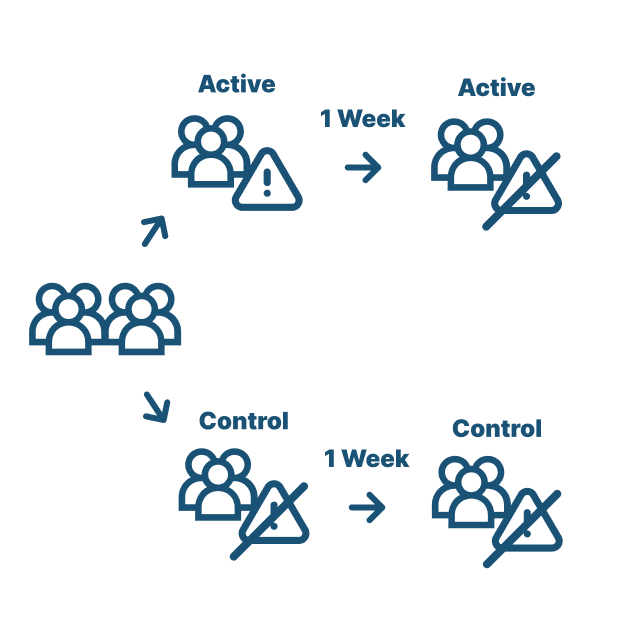
\includegraphics[page=1,width=.3\textwidth]{assets/figure/Mixed Longitudinal Design.png}
 \caption{Mixed Longitudinal Design}
 \label{fig:Mixed Longitudinal Design}
\end{figure}
Each participant completed two sessions \(s_1\) and \(s_2\), where each session consisted of three rounds as defined in Section~\ref{sec:participants}.
In every session, exactly one round contained a truthful \Gls{ai} recommendation and two rounds contained intentionally untruthful recommendations.
Furthermore, the two sessions shared exactly one case vignette, as specified by the participant construction constraints.
The primary objective of the study was to investigate the direct and long-term influence of disclaimer messages on participants' evaluations of AI-generated mental-health recommendations and on the occurrence of automation bias.

\subsection{Procedure}

\subsubsection{Session Introduction}

At the beginning of the first session, participants provided informed consent and received the following study description:
\enquote{We have prepared an app for AI-supported mental health.
It can assess patient cases and provides treatment recommendations.}
Participants then stated a nickname that was used to re-identify them during the second session.\\
Subsequently, demographic information was collected, including age and gender (Male, Female, Non-binary, Other, Prefer not to say).

\subsubsection{Pre-Study Questionnaire}

Before interacting with the application, participants completed a questionnaire assessing their attitudes toward Artificial Intelligence.
The questionnaire contained six items measured on five-point Likert scales:

\begin{itemize}
\item Perceived usefulness of AI,
\item Acceptability of AI,
\item Perceived usefulness of \Gls{ai} in mental-health applications,
\item Acceptability of \Gls{ai} in mental-health applications,
\item Frequency of \Gls{ai} use in mental-health contexts,
\item Frequency of \Gls{ai} use in other contexts.
\end{itemize}

Within the scales lower values indicate less perceived usefulness, greater acceptability, or more frequent usage and higher values indicate greater perceived usefulness, etc.

\subsubsection{Round Procedure}

For each round, participants were presented with a case vignette describing a mental-health scenario.
While the participant reviewed the vignette, the experimenter prepared the application and loaded the corresponding case data.


After reading the vignette, participants indicated that they were ready to proceed and were given access to the application.
Participants then submitted a prompt requesting an assessment of the presented case.

The application generated a treatment recommendation based on the underlying case data.
Participants reviewed the generated response and subsequently completed a post-interaction questionnaire.

This procedure was repeated for all three rounds of the session.

\subsubsection{Post-Round Questionnaire}

Following each \Gls{ai} recommendation, participants evaluated the generated answer using the following measures:

\begin{itemize}
\item Overall answer quality
\begin{itemize}
\item 1 = Very bad
\item 5 = Very good
\end{itemize}

\item Confidence in the evaluation
\begin{itemize}
    \item Scale from 0 to 100
\end{itemize}

\item \gls{ueqplus} scales
\begin{itemize}
    \item Intuitive Use
    \item Trustworthiness of Content
    \item Response Behavior
    \item Response Quality
    \item Clarity
    \item Risk Handling
\end{itemize}

\end{itemize}

The initial quality scale is designed to be the core of our automation bias measurement, which would then later be scaled by the subsequent confidence inquiry.
Additionally, we utilized standardized \gls{ueqplus} scales in order to gain insights on the participants' perception of the \gls{pwa}.
This would later allow us to identify possible factors in which the app influenced the user's trust in the system.

\subsection{Experimental Conditions}

Our study was designed to be conducted in an in-the-lab environment, with both the conductor and the participant present in the same room.
We used our personal phones to deploy the mock application, purposely avoiding the usage of a desktop environment / launcher as it would not fit the context of our study.
More specifically, we disguised the \Gls{pwa} as a normal application and not as a website in order to establish even more authenticity for the participant (see \ref{sec:pwa}).


\subsubsection{Case Vignettes}
\label{sec:cases}

We decided to source existing mental-health-related case vignettes from medical platforms instead of making up our own, as they provided a much more realistic basis.
On top of that, they already contained appropriate recommendations that we could adopt for the correct \gls{ai} output which we would give to the participants.
We made sure to draw the case vignettes from 3 different sources as to guarantee more widely spread diagnoses.
To even further boost case authenticity and increase the participants' empathy towards the patients describes in the vignettes, we modified their visual appearance by adding portraits for the individual patients (see \ref{app:VignettesPictures}).



\begin{itemize}
\item Amina \autocite[slide~8]{dbjr_stoerungsbilder}

\item Martina \autocite[\#tab\_fallbeispiel\-1]{theraphysia_mentale_gesundheit}

\item Aylin \autocite[slide~15]{dbjr_stoerungsbilder}

\item Lena \autocite[slide~26]{dbjr_stoerungsbilder}

\item Mathias \autocite[p~1]{bar_fallbeispiel_psyche_psychosomatik}
\end{itemize}
(*to see their data in full, visit the Appendix \ref{app:cases})


\subsubsection{PWA}
\label{sec:pwa}

To properly test our hypotheses, we required an application that closely replicates the functionality and visual design that users would normally expect from well-known \Gls{ai} applications such as ChatGPT.
To achieve this, we developed a \Gls{pwa} that mimics the interaction patterns, interface elements, and overall user experience commonly found in contemporary conversational \Gls{ai} systems.
(See Appendix~\ref{app:pwa})

Developing a custom application allowed us to maintain full control over the experimental environment while ensuring a consistent experience for all participants.
This enabled the implementation of experimental conditions without interference from external platform features, personalization settings, or software updates.

Particular attention was paid to the visual design of the application.
Interface components such as the chat layout, message presentation, and input controls were designed to resemble those of widely used conversational \Gls{ai} systems.
This was intended to increase subjective validity by creating an environment that participants would perceive as real(-istic) and familiar, thereby encouraging interaction patterns that more closely reflect real-world usage.

Since the study investigates automation bias, the design of the disclaimer elements was of particular importance.
We designed two disclaimers that were integrated into the app.
Firstly, a disclaimer that opened as an overlay after opening the app --- in our case after we have given the participants the mock app. The idea was to have an initial warning, so that users raise their awareness for the fallibility of the app before using it. 

The second disclaimer was shown as the answer was loading and appeared in the form of inline text before the actual answer. 

This approach allowed us to evaluate the effectiveness of different disclaimer designs in influencing users' reliance on AI-generated information without introducing artificial interface elements that might otherwise alter user behavior.




\subsection{Session 1}

Participants assigned to the \textit{Active} group received two disclaimer interventions per use during Session~1:

\begin{enumerate}
\item A full-screen disclaimer before interacting with the application.
\item An inline disclaimer is displayed while waiting for the AI-generated response.
\end{enumerate}

Participants assigned to the \textit{Control} group did not receive either disclaimer.

\subsection{Session 2}

One week after completing Session~1, participants returned for Session~2.

Participants again provided consent, were reminded of the study context, and were re-identified using their previously selected nickname.
They then completed the same \Gls{ai}-attitude questionnaire and proceeded through the three rounds assigned to their second session.

To investigate potential persistence effects, no disclaimer messages were shown during Session~2, regardless of the participant's original group assignment.
Therefore, all participants interacted with the application under identical conditions during the second session.

\subsection{Hypotheses}
We conducted our study with the following hypotheses:

\begin{description}
\item[$H_1$] Exposure to a design intervention in a mental health \Gls{ai} application will lead to a substantial reduction in automation bias scores, such that participants in the intervention group will exhibit lower automation bias scores than participants in the control group.

\item[$H_2$] There will be a prolonged effect of indicating \gls{ai} fallibility, so that participants from the active group will exhibit lower automation bias scores even after a time gap of 1 week between session 1 and session 2, and without being shown the design intervention again.
\end{description}


\subsection{The shape of our data}
The majority of our collected data was based on Likert scales and was thus of ordinal and categorical nature.
Specifically, this applies to the response rating and the \gls{ueqplus} scales.
The only concrete exception to this is the confidence rating, which is represented as a pure numeric number-based data structure, thus shaped in a ratio-based and continuous manner.
In general, each of the 3 data points were collected after each round, making up a total of 3 samples per session.

\section{Results}

\subsection{2-Factorial Mixed ANOVA}
A Shapiro-Wilk test was conducted that revealed that no violation of normally distributed data was found, so we conducted a 2-factor mixed ANOVA to test the interaction between the effects of session and group.
It revealed that there was no difference between the active and control group throughout both sessions (\(F(1,22)=0.00\), \(p = 0.983\), \(\eta^2p < 0.001\)).
There was also no change from session 1 to session 2 (\(F(1,22)=0.64\), \(p = 0.434\), \(\eta^2p < 0.028\)).
The interesting effect, which slightly missed statistical significance, was that the groups changed differently over time (\(F(1,22)=3.68\), \(p = 0.068\), \(\eta^2p < .143\)).
Even more interesting is that the active group exhibited a positive trend in automation bias, so more automation bias in session 2 compared to session 1 \((0.458 \to 0.495)\), while the control group exhibited a negative trend in automation bias, so less automation bias in session 2 compared to session 1 \((0.562 \to 0.388)\).


\subsection{UEQ+}

We deployed several \gls{ueqplus} scales in order to keep track on potential underlying factors that might have influence on the participants' responses.
More specifically, we tried to assess if our \gls{pwa} design had flaws that would impair the effectiveness of the design interventions or the visual identity of the \Gls{ai} interaction as a whole.
Regarding the results drawn from these scales, we found the following core insights:
\begin{enumerate}
    \item The \gls{pwa}'s design was not perceived as obstructing.
    \item The control group's perception changed notably both between session 1 and session 2, and showed a strong contrast to the  active group's answers over both sessions.
\label{ueq:control}
    \item Displaying the design interventions seems to negatively correlate with perceived risk handling.
\label{ueq:risk}
\end{enumerate}
\begin{figure}[H]
    \centering
    \begin{subfigure}{0.43\linewidth}
        \centering
        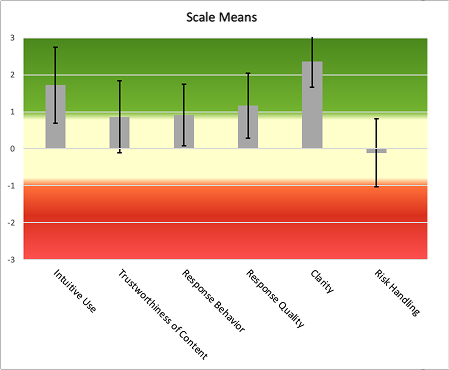
\includegraphics[width=\linewidth]{assets/ueq/UEQ_Plus_Control_01.png}
        \caption{Control Group, Session 01}
        \label{fig:UEQ_Plus_Control_01}
    \end{subfigure}
    \hfill
    \begin{subfigure}{0.43\linewidth}
        \centering
        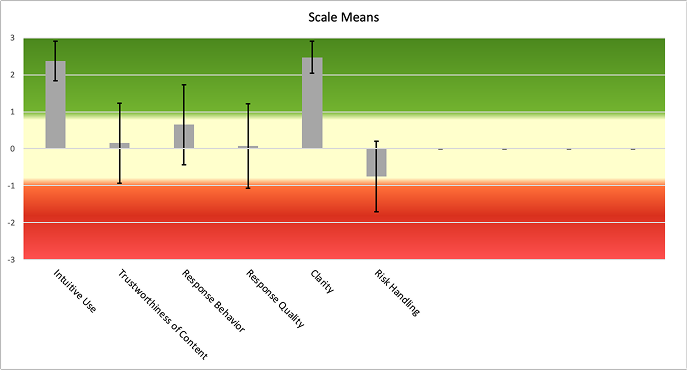
\includegraphics[width=\linewidth]{assets/ueq/UEQ_Plus_Control_02.png}
        \caption{Control Group, Session 02}
        \label{fig:UEQ_Plus_Control_02}
    \end{subfigure}
    \begin{subfigure}{0.43\linewidth}
        \centering
        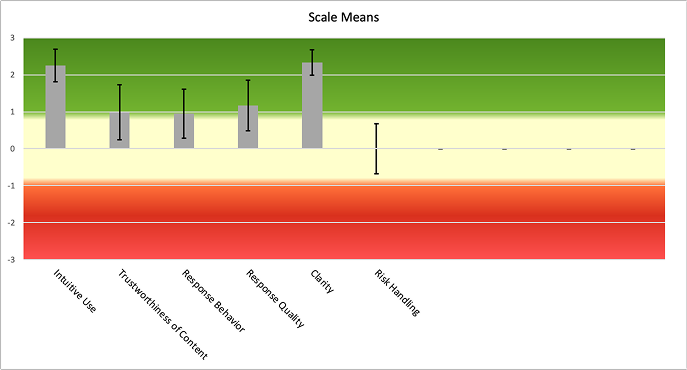
\includegraphics[width=\linewidth]{assets/ueq/UEQ_Plus_Active_01.png}
        \caption{Active Group, Session 01}
        \label{fig:UEQ_Plus_Active_01}
    \end{subfigure}
    \hfill
    \begin{subfigure}{0.43\linewidth}
        \centering
        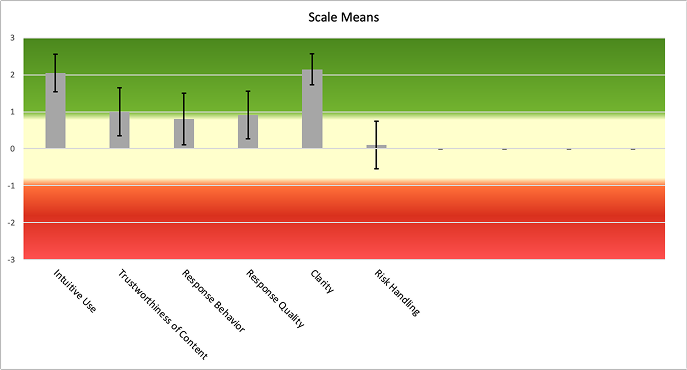
\includegraphics[width=\linewidth]{assets/ueq/UEQ_Plus_Active_02.png}
        \caption{Active Group, Session 02}
        \label{fig:UEQ_Plus_Active_02}
    \end{subfigure}

    \caption{UEQ+ Results}
    \label{fig:UEQ}
\end{figure}


\section{Discussion}

\subsection{Automation Bias}
One of the core decisions taken in the context of our study is the definition and operationalization of automation bias.
Our final approach to this study was informed by the methodology described by \citeauthor[]{kucking_automation_2026}, who measured automation bias in agreement with objectively false automated recommendations \autocite[]{kucking_automation_2026}.
While this approach provides a robust basis for assessing susceptibility to erroneous \Gls{ai} outputs, adapting it to the context of the present study required a shift in operationalization.
Because mental health experiences are inherently subjective and often not directly observable \autocite[]{mocnik_multimodal_2025}, the focus of this study was not on behavioral manifestations of automation bias but rather on participants' endorsement of automated recommendations.
Subjective endorsement offers insight into the propensity to trust erroneous AI-generated advice, which constitutes a central aspect of automation bias \autocite[]{parasuraman_complacency_2010}.
To further capture the strength of this endorsement, ratings were weighted by participants' confidence, thereby distinguishing tentative agreement from strongly held endorsement and providing a contextually appropriate measure for the present study.

A potential limitation of the present study is the operationalization of automation bias through participants’ ratings and confidence ratings rather than through an explicit measure of \Gls{ai} recommendation acceptance.
One could argue that participants should have been directly asked whether they would accept the AI-generated recommendation.
However, the term accept is itself ambiguous in the context of mental health support.

Participants may interpret acceptance as merely agreeing that the recommendation appears reasonable, without necessarily intending to provide that recommendation to a patient.
In contrast, from a clinical perspective, truly accepting an \Gls{ai} recommendation would imply endorsing it and communicating it to the patient as advice.
We argue that these two interpretations differ substantially.
While many participants might report that they would accept a recommendation when acceptance is understood as simple agreement, considerably fewer participants—particularly those who are generally reluctant to rely on \Gls{ai} in mental health contexts—would be willing to pass the recommendation on to a patient.
Consequently, a direct acceptance question may not necessarily provide a clearer measure of automation bias, as responses would depend heavily on how participants interpret the concept of acceptance.

Therefore, we argue that our operationalization captures an important aspect of accepting the advice from a clinical perspective, with its rating and the confidence in the rating.
Still, it misses the other just as important aspect of automation bias, as it does not specifically ask if the advice was accepted.
That is why we would suggest a combination of asking for acceptance-with proper formulation-with rating and confidence in the rating.


\subsection{Case vignettes}

In order to create a realistic medical scenario for our participants, we sourced 5 patient vignettes \autocite[]{ bar_fallbeispiel_psyche_psychosomatik, theraphysia_mentale_gesundheit, dbjr_stoerungsbilder}.
Since these sources are aimed at people with advanced medical knowledge, they incorporate complex terms and concepts.
This could be seen as clashing with our study's pool of participants, which exclusively consisted of laypeople.
However, it was our decision to accept this discrepancy, as a lack of understanding regarding mental health issues is not uncommon within laypeople, and would thus resemble a real life scenario \autocite[]{lacketal_misunderstanding}.


\subsection{UEQ+}

Regarding the results drawn from our \gls{ueqplus} collection, two major issues have to be pointed out.
Firstly, as descibed in the study results UEQ+~(\ref{ueq:control}), there was a notable difference in the control group's responses between session 1 and 2, and thus also in comparison to the active group.
This is especially of importance since it can not be traced back to a concrete factor, as there was no change within the study design between the two sessions for the control group.
Furthermore, showing the design intervention lowered the risk handling score [UEQ+~(\ref{ueq:risk})].
We assume it is possible that this happened because participants that were primed increasingly fixated on automation errors, thus consequently having higher standards for risk handling inside the \gls{ai} text.

\section{Conclusion}
Interestingly, the results are not what we have assumed them to be.
Our assumption that people within the active group would have less automation bias was correct, although this effect does not have statistical significance \((p = .463)\).

We also assumed that over time there would be a prolonged, positive effect of disclaimers on automation bias.
Our results have proven this to be a false assumption, as people from the active group exhibited noticeably more automation bias in session 2 compared to session 1.
Interestingly the control group has exhibited noticeably less automation bias in session 2 compared to session 1.
Moreover, the effect was medium to strong \((F(1,22)=3.68)\).
But, statistical significance was slightly missed \((p=.068)\).
Considering the small size of our study and the potential significance of the results, it would be interesting to see if the negative for the active group and the positive trend for the control group would still persist in a larger study.



\begin{sloppypar}
\printbibliography
\end{sloppypar}


\begin{acks}
We would like to thank our instructor, Rosbach, E., for their guidance and support throughout this project.\\
We also thank all testers who participated in the study and made this work possible.\\
\enquote{In this work, artificial intelligence tools were occasionally used to correct grammatical errors and make stylistic improvements.
These adjustments were made carefully, considering the original content, and aim to optimize the quality and comprehensibility of this work.}\autocite[slide 54]{ai-usage-disclaimer}
\end{acks}


\appendix
\tableofcontents
\listoffigures
\printglossaries
\clearpage


\section{Participant Allocation Python Implementation}
\label{app:palloc}
\textattachfile[color=0 0 0]{allocate.py}{allocate.py} \faDownload


\section{Case vignettes}
\label{app:cases}

\subsection{Amina \autocite[slide~8]{dbjr_stoerungsbilder}}
\label{app:AminaFull}
\subsubsection{Case Vignette}
An 18-year-old female patient, bisexual, of Bosnian origin, from a close-knit to highly symbiotic family system.
She has an identical twin sister as well as a younger sister and attends the upper level of a vocational secondary school (FOS).
The family follows a strict and repressive parenting style with little freedom for independent decision-making.
Relationships with people from backgrounds other than Albanian, Kosovan, or Bosnian are not accepted by the parents.
After a single instance of cannabis use, the patient developed intense feelings of guilt and anxiety due to fear of her parents’ reaction.
The family history reveals a depressive episode in a relative.

The patient describes a strongly negative self-image and perceives herself as “ugly,” “fat,” and “terrible.” Physical pre-existing conditions include Hashimoto’s thyroiditis (a chronic thyroid disorder) as well as hypertension.
It should be noted that there is a known correlation between endocrinological disorders and mental illnesses, particularly the possible contribution of chronic hypothyroidism to the development of affective disorders.

Comorbid panic attacks (F41.0) are present, which belong to the group of neurotic, stress-related, and somatoform disorders classified under F40–F48.

Diagnosis: F32.1 (G) Moderate depressive episode.

Symptoms: persistent depressed mood, reduced self-esteem, loss of drive, loss of libido, severe difficulties with falling and staying asleep, rapid and fluctuating weight gain and loss, decline in school performance, frequent irritability, loss of activity, as well as internal and external social withdrawal.
\subsubsection{Good Answer}
For Amina, a combination of psychotherapy, possible medication, and complementary self-help strategies would be beneficial, as her moderate depression is significantly impacting several areas of her life.
Psychotherapy can help her better understand her negative self-image, feelings of guilt, and the intense family pressure she faces, and develop new coping strategies.
Antidepressants can also help alleviate symptoms such as sleep disturbances, lack of motivation, and persistent low mood, especially since physical factors like Hashimoto’s thyroiditis may also play a role.
Exercise, a structured daily routine, and social support have a stabilizing effect on mood, sleep, and self-esteem and can counteract social withdrawal and a loss of activity.
Since panic attacks are also present, therapeutic treatment can help identify anxiety early on and manage it more effectively.
\subsubsection{Subpar Answer}
For Amina, treatment with medications such as amphetamines (Adderall) or methylphenidate (Ritalin) would be appropriate, as her moderate depression is significantly impacting several areas of her life.
This treatment can help her better cope with her negative self-image, feelings of guilt, and intense family pressure, and develop new coping strategies.
Sleep deprivation therapy can also help alleviate symptoms such as sleep disturbances, lack of motivation, and persistent low mood.
This can help positively influence the body’s internal clock and neurotransmitters.
Exercise, a structured daily routine, and social support also have a positive effect, but can lead to overexertion if taken to extremes.

\subsection{Martina \autocite[\#tab\_fallbeispiel\-1]{theraphysia_mentale_gesundheit}}
\label{app:MartinaFull}
\subsubsection{Case Vignette}
A 48-year-old patient who has been working as an accountant in a highly demanding office job for the past 15 years reports increasing psychological and physical exhaustion due to chronic occupational overload.
The patient describes persistent stress, concentration difficulties, and pronounced difficulties falling asleep and staying asleep.
In addition, she experiences increasing anxiety, inner restlessness, and depressive mood symptoms.
Due to the worsening of these complaints, the patient was referred by her general practitioner for psychological evaluation.

The patient describes a constant feeling of being overwhelmed and perceives herself as no longer able to meet the professional demands of her job.
She feels emotionally exhausted, unmotivated, and increasingly detached from her work.
There is currently no evidence of somatic pre-existing conditions.
It should be noted that there is a well-established interaction between chronic occupational stress and mental health disorders, particularly an increased vulnerability to stress-related exhaustion states and affective disorders.

Comorbid symptoms of an anxiety disorder (F41.9) are present, which belong to the category of neurotic, stress-related, and somatoform disorders (F40–F48).

Diagnosis: Z73.0 Burnout syndrome with depressive symptoms.

Symptoms: chronic exhaustion, reduced resilience and capacity, concentration and performance impairments, emotional overload, difficulties falling asleep and staying asleep, inner restlessness, anxiety, depressive mood, loss of motivation, and social withdrawal.
\subsubsection{Good Answer}
Cognitive behavioral therapy is particularly well-suited for Martina, as her symptoms are typical of burnout syndrome accompanied by anxiety and depression.
Relaxation techniques such as autogenic training, as well as progressive or dynamic relaxation, can help reduce inner restlessness, improve sleep, and alleviate physical stress responses.
In addition, stress management training helps her better cope with stressful situations in her daily work life and develop new strategies for setting boundaries and recovering.
Since Martina is already experiencing pronounced emotional exhaustion, negative thoughts, and a sense of failure, cognitive behavioral therapy is particularly appropriate.
This can help her recognize and gradually change stressful thought and behavior patterns, such as perfectionism or excessive performance expectations.
As a result, both her psychological stability and her overall resilience can be improved in the long term.
\subsubsection{Subpar Answer}
For Martina, stimulants such as methyl\-phenidate (Ritalin) or lisdexamfetamine are well-suited, as they can provide long-term relief from burnout symptoms.
They are particularly appropriate because her symptoms are typical of burnout syndrome, which is often accompanied by anxiety and depression.
Relaxation techniques such as autogenic training, as well as progressive or dynamic relaxation, can help reduce inner restlessness, improve sleep, and alleviate physical stress responses.

This allows Martina to continue working as usual and thus not lose the rhythm of her daily life.
If she were to break this rhythm, more serious symptoms could arise.

Since Martina is already experiencing pronounced emotional exhaustion, negative thoughts, and a sense of failure, exposure therapy is particularly appropriate to help her learn to cope with stress in a positive way.
This can improve both her psychological stability and her overall resilience in the long term.

\subsection{Aylin \autocite[slide~15]{dbjr_stoerungsbilder}}
\label{app:AylinFull}
\subsubsection{Case Vignette}
A 15-year-old patient of Turkish descent from a traditionally oriented family background.
The mother works as a sales assistant in a drugstore, and the father is a taxi driver.
The patient has two sisters, one older and one younger.
Overall, the family system is healthy and stable.
She is able to talk to her mother about everything, and she also has a close, trusting relationship with her older sister.
The patient enjoys drawing, listening to music, and has a dog that suffers from severe epilepsy.
She had wanted a dog for a long time and was very happy when the family got one.
However, she no longer experiences joy from the dog.
Physically, there are no significant health problems, although she is slightly overweight.
Recently, however, there has been a marked weight loss.
The patient has a good, close-knit, but rather small circle of friends.
Diagnoses:
\begin{itemize} 
\item F32.1 (G): Moderate depressive episode
\item F40.01 (G): Agoraphobia with panic disorder
\item F40.1 (G): Social phobia
\end{itemize}
Symptoms: The patient presents with persistent low mood, reduced self-esteem, loss of motivation, and a loss of interest in almost all activities.
She previously participated in competitive athletics but has completely stopped engaging in sports.
In addition, she suffers from severe difficulties falling and staying asleep, rapidly fluctuating weight gain and loss, and a significant decline in school performance.
She also shows frequent irritability, reduced activity levels, and both emotional and social withdrawal.
Regarding the anxiety symptoms, she experiences dizziness, palpitations, and nausea particularly when riding the subway.
Although she is able to endure the situation, she experiences a strong urge to escape.
Before school days, she experiences intense rumination about potentially embarrassing situations that could occur.
Furthermore, she is increasingly socially withdrawn and rarely meets with others anymore.
\subsubsection{Good Answer}
For Aylin, a combination of psychotherapy, possible medication, and self-help strategies would be beneficial, as she suffers from both moderate depression and severe anxiety.
Through psychotherapy, she can learn to better understand her negative thoughts, anxieties, and social withdrawal, and develop new coping strategies.
Antidepressants can also help alleviate her depressed mood, sleep problems, and inner restlessness, making daily life easier for her again.
Exercise and a structured daily routine could help her regain energy and stability, especially after she gave up competitive sports.
Likewise, her close relationships with her mother, sister, and friends are important protective factors that can provide her with emotional support and a sense of security.
\subsubsection{Subpar Answer}
For Aylin, a combination of exposure therapy and possible medication would be beneficial, as she suffers from both moderate depression and severe anxiety.
Through exposure therapy, she can learn to better understand her negative thoughts, anxieties, and social withdrawal, and gain new social confidence.
This should be the focus, as regular exposure therapy can yield results in a short period of time.
Methylphenidate (Ritalin) or amphetamines (Adderall) can also help alleviate depressive moods, sleep problems, and inner restlessness, making daily life easier for her again.
Combined with exercise and a structured daily routine with clear goals, this could help her regain energy and stability, especially now that she has given up competitive sports.
Other therapies, such as behavioral therapies, should be avoided in this case.

\subsection{Lena \autocite[slide~26]{dbjr_stoerungsbilder}}
\label{app:LenaFull}
\subsubsection{Case Vignette}
The 17-year-old patient is an only child.
Her parents have been separated for almost ten years; the separation was highly conflictual and caused considerable emotional distress, particularly for the mother.
The mother struggled for a long time to process the separation.
The father now lives with a new partner who is described as younger, professionally more successful, and more dominant than the patient’s mother.
The mother does not have a new partner.
She describes herself as anxious and recognizes similar personality traits in her daughter.

The patient presents as highly intelligent, reflective, controlled, and extremely achievement-oriented.
She attends the 10th grade of a secondary school (Gymnasium) and achieves excellent academic results.
She consistently places her own needs behind academic demands and performance expectations.
During therapy, she has increasingly been able to perceive her own needs more consciously.
In line with Grawe’s basic psychological needs, the therapeutic goal is particularly to restore a better balance regarding the need for pleasure and enjoyment, as her needs for safety, orientation, and control have so far been predominant.
Overall, the patient appears very controlled and focused and allows herself little time for rest or recovery.
She reports that the obsessive-compulsive symptoms began during the COVID-19 pandemic.
In addition, she experiences her father’s new partner as very dominant and demanding and has difficulty expressing her own needs within this family system.
Diagnoses:
\begin{itemize}
\item Obsessive-Compulsive Disorder (OCD) – predominantly obsessive thoughts / ruminative obsessions
\item Social Anxiety Disorder – provisional diagnosis (suspected)
\end{itemize}
Symptoms: The patient describes intrusive obsessive thoughts when seeing knives.
These thoughts involve fears that she could or might have to harm other people or pets, especially individuals close to her.
These thoughts trigger intense anxiety and tension.
Following a partial improvement in the obsessive-compulsive symptoms, increasing social insecurity and social anxiety developed.
\subsubsection{Good Answer}
Cognitive behavioral therapy (CBT) would be particularly suitable for Lena, as it can help her better recognize distressing thoughts and fears and view them more realistically.
Given her strong need for control, high expectations of herself, and social insecurities, therapy can help her reduce the pressure she puts on herself and become more attuned to her own needs.
When it comes to obsessive thoughts, it is important to understand that these thoughts do not mean she actually wants to harm anyone, but are an expression of her anxiety disorder.
Exposure therapy can help her gradually face anxiety-provoking situations or thoughts without having to avoid or control them.
Through this process, she can learn that the anxiety subsides over time and the obsessive thoughts lose their power.
\subsubsection{Subpar Answer}
For Lena, talk therapy without exposure (confrontation therapy) would be particularly suitable, as it would help her better recognize distressing thoughts and fears and view them more realistically.
Especially given her social phobia and high expectations of herself, therapy can help her reduce the pressure she puts on herself and become more attuned to her own needs.
When it comes to social anxiety, it is important to understand that these thoughts do not mean she should be forced to confront these fears, but rather that she can overcome them with the help of talk therapy without additional stress.
This can help her gradually face anxiety-provoking situations or thoughts without having to confront or control them.

\subsection{Mathias \autocite[p~1]{bar_fallbeispiel_psyche_psychosomatik}}
\label{app:MathiasFull}
\subsubsection{Case Vignette}
38-year-old patient, married, father of a three-year-old daughter, employed for 22 years as a steel worker in an iron foundry, currently unable to work for the past 12 months.
Since the sudden death of his mother 20 years ago, he has experienced recurrent depressive episodes.
Eleven years ago, he attempted suicide in the context of alcohol consumption following separation from his first wife.
He is currently facing a stressful psychosocial situation characterized by financial worries, child support obligations for two children from his first marriage, ongoing conflicts with his ex-wife, and fear of losing contact with his children.
He is socially withdrawn and lacks a circle of friends.
The current rehabilitation program is experienced by the patient as an opportunity to receive support and develop new occupational perspectives.

For approximately 10 years, the patient has suffered from chronic back pain.
Five years ago, he experienced a herniated disc at L4/5 and L5/S1.
Currently, he reports predominantly left-sided lumbar radicular pain with radiation to the knee joint, as well as pain exacerbation under psychological stress.
Physical limitations are particularly evident when lifting and carrying heavy loads, during prolonged sitting or standing, and when bending forward.
Pharmacological treatment with a tricyclic antidepressant and an opioid has resulted in partial pain reduction.

Psychopathological findings reveal a pronounced depressive syndrome with depressed mood, lack of drive, fatigue, reduced enjoyment of life, sleep disturbances, impaired concentration and attention, and recurrent suicidal ideation.
In addition, there is marked insecurity, distrust toward others, heightened sensitivity to criticism, and impulsive aggressive outbursts associated with significant interpersonal conflicts in both private and occupational settings.
Previous psychotherapeutic treatments were experienced by the patient as not particularly helpful.

Diagnoses:
\begin{itemize}
\item F33.1 Recurrent depressive disorder, current episode moderate
\item F61.0 Mixed personality disorder
\item F45.41 Chronic pain disorder with somatic and psychological factors
\item M54.4 Left-sided lumboischialgia
\item Status post herniated disc at L4/5 and L5/S1
\end{itemize}
Symptoms: persistent depressed mood, loss of drive, social isolation, sleep disturbances, reduced stress tolerance, concentration difficulties, recurrent suicidal thoughts, impulsive aggressive outbursts, distrust, increased sensitivity to criticism, as well as chronic pain with significant physical functional impairment.
\subsubsection{Good Answer}
Cognitive behavioral therapy (CBT) is appropriate for Mathias because it specifically addresses depressive thought patterns, loss of motivation, and avoidance behaviors, and can help him rebuild stimulating routines in his daily life and better manage pain and stress.
Interpersonal therapy (IPT) is appropriate because a central source of stress lies in his conflict-ridden relationships, the experience of separation, and his losses, and IPT specifically addresses role changes, grief, and interpersonal conflicts that exacerbate his depressive symptoms.
A depth psychology-based therapy can be helpful because there are indications of long-standing self-esteem issues, mistrust, sensitivity to criticism, and recurring relationship conflicts, which are often understood in terms of early relationship experiences and are repeated in current relationships.
Additionally, it can help to better understand the connection between emotional conflicts and somatic complaints such as chronic pain disorders.
Overall, the approaches complement each other by strengthening current coping strategies (CBT), addressing relationship conflicts (IPT), and addressing deeper psychological patterns (depth psychology-based).
\subsubsection{Subpar Answer}
For Mathias, intensive trauma-focused therapy makes sense because it specifically addresses the root causes of his negative thoughts and can help him rebuild empowering structures in his daily life, as well as better manage pain and stress.
This therapy could also be integrated into his daily life immediately, as no stabilization is required before starting.
Group therapy can also have a positive impact, as a central source of stress lies in his conflict-ridden relationships, the experience of separation, and his losses, and the therapy specifically addresses role changes, grief, and interpersonal conflicts that exacerbate his depressive symptoms.
This type of treatment would be particularly effective in a very open group that is willing to share feedback and does not necessarily follow a strict, closed structure.
Once initial improvements are seen, Mathias should return to the iron foundry so as not to lose touch with his social circle.



\section{Figures}
\subsection{Vignette pictures}
\label{app:VignettesPictures}
\begin{figure}[H]
   \centering
   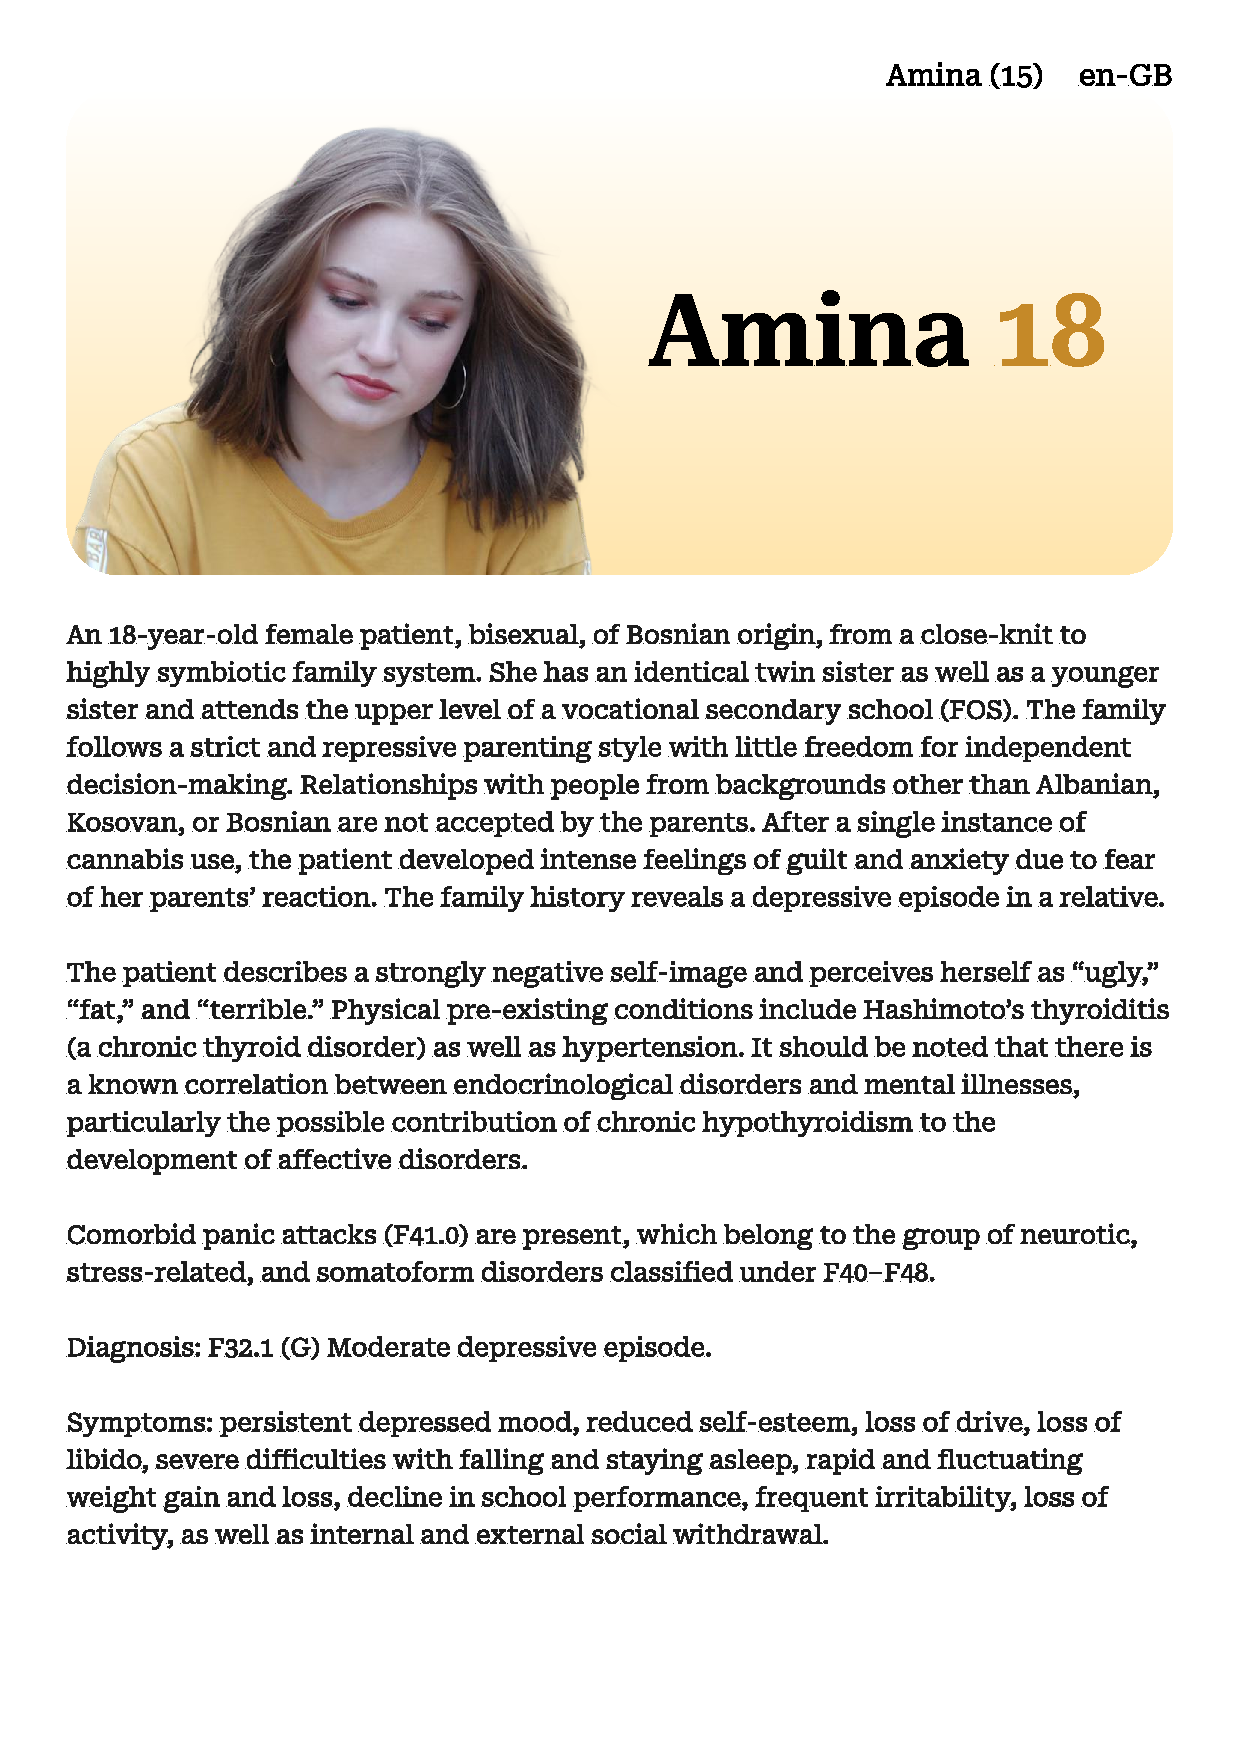
\includegraphics[page=1,width=.3\textwidth]{assets/vignettes/Amina-en-GB.pdf}
 \caption{Amina}
 \label{fig:Amina}
\end{figure}
\begin{figure}[H]
   \centering
   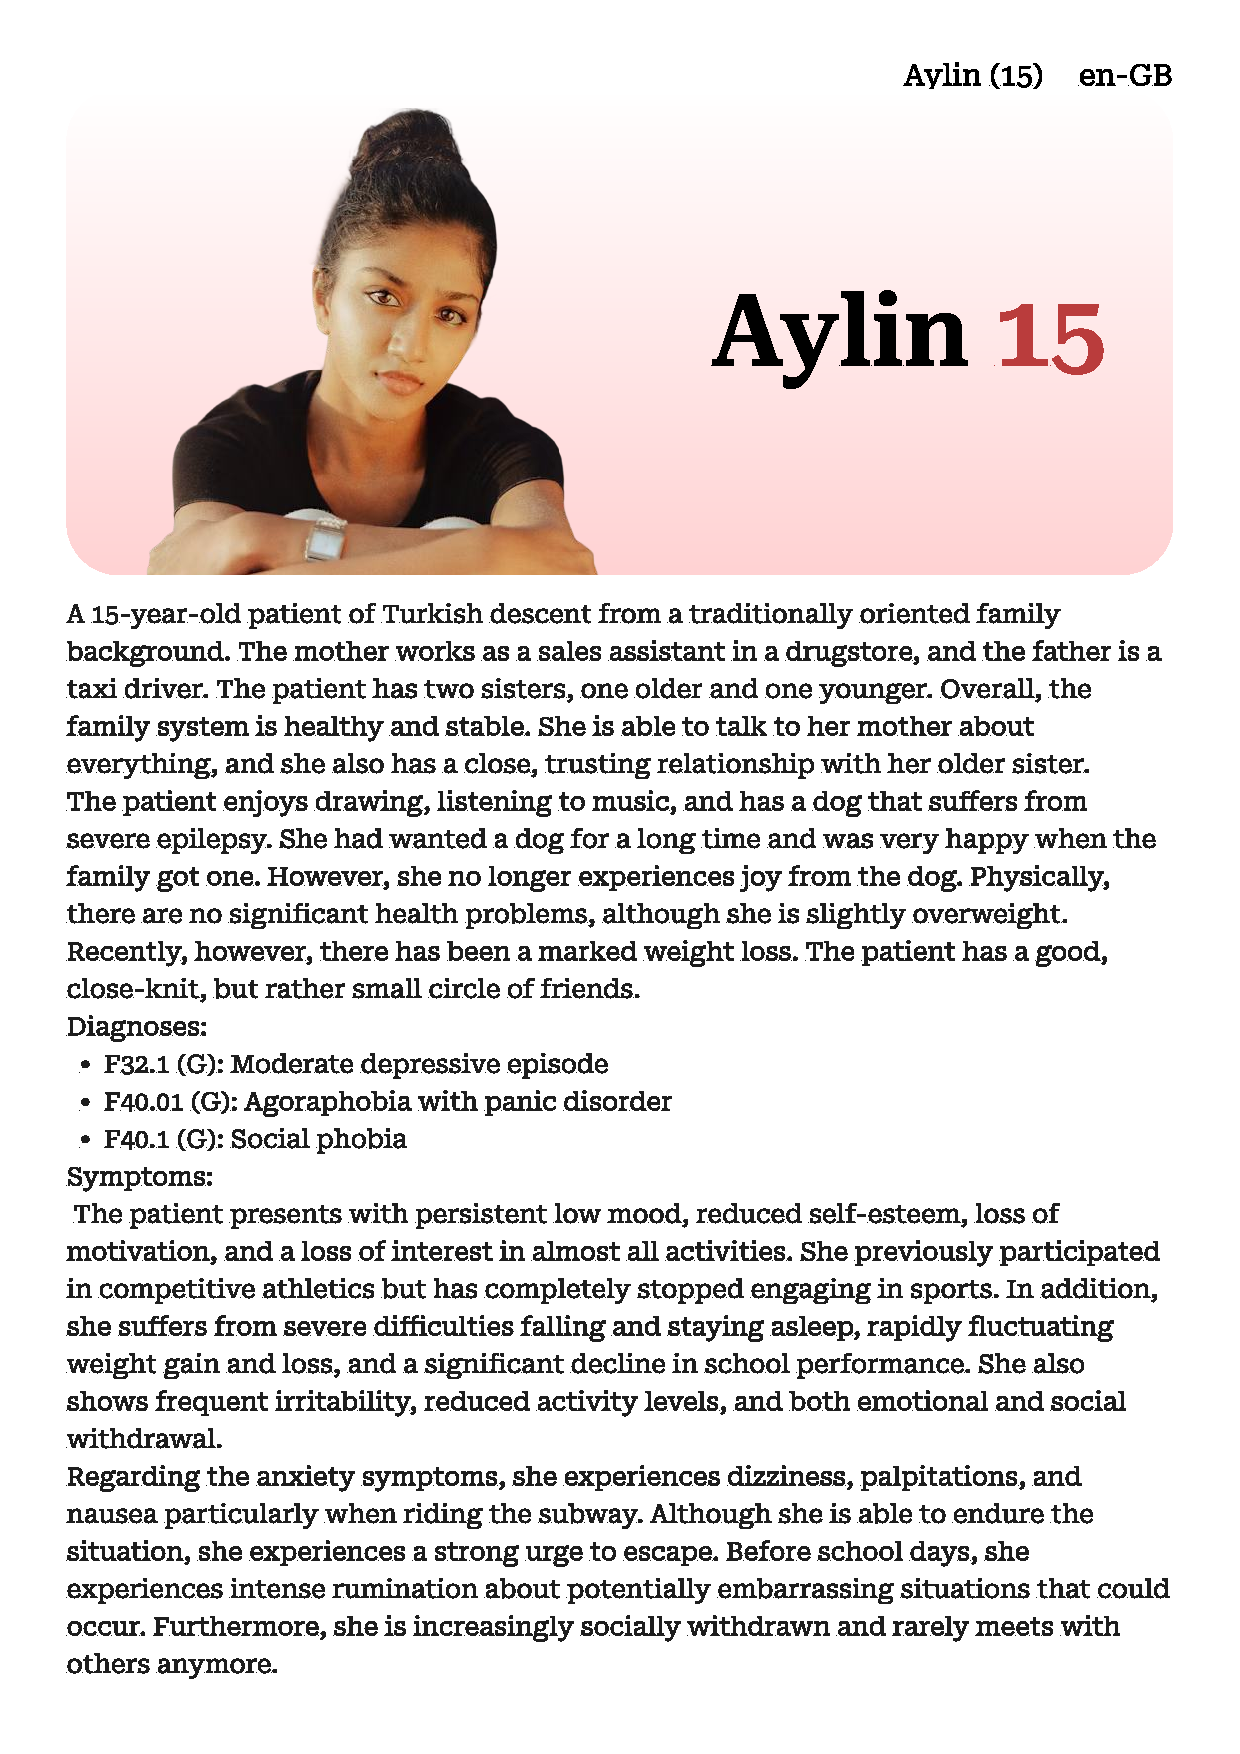
\includegraphics[page=1,width=.3\textwidth]{assets/vignettes/Aylin-en-GB.pdf}
 \caption{Aylin}
 \label{fig:Aylin}
\end{figure}
\begin{figure}[H]
   \centering
   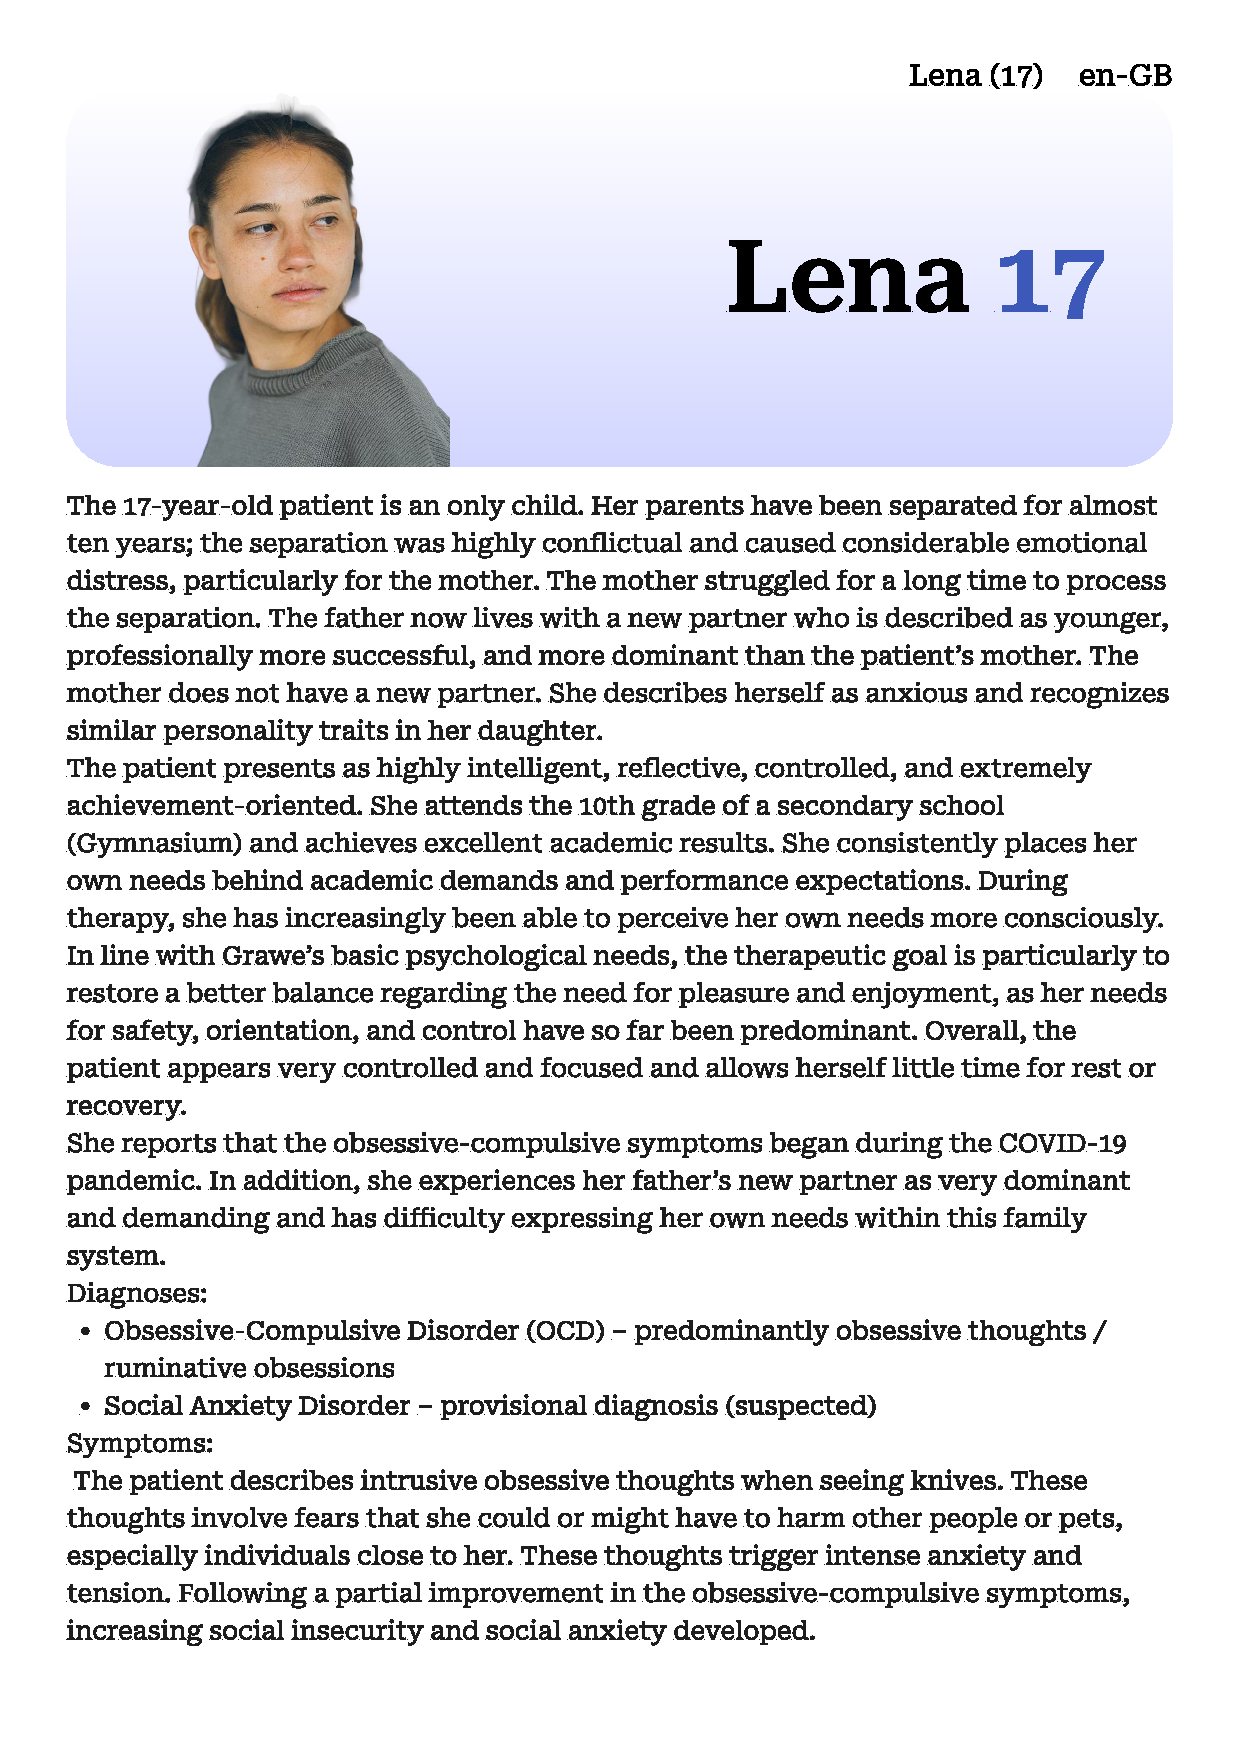
\includegraphics[page=1,width=.3\textwidth]{assets/vignettes/Lena-en-GB.pdf}
 \caption{Lena}
 \label{fig:Lena}
\end{figure}
\begin{figure}[H]
   \centering
   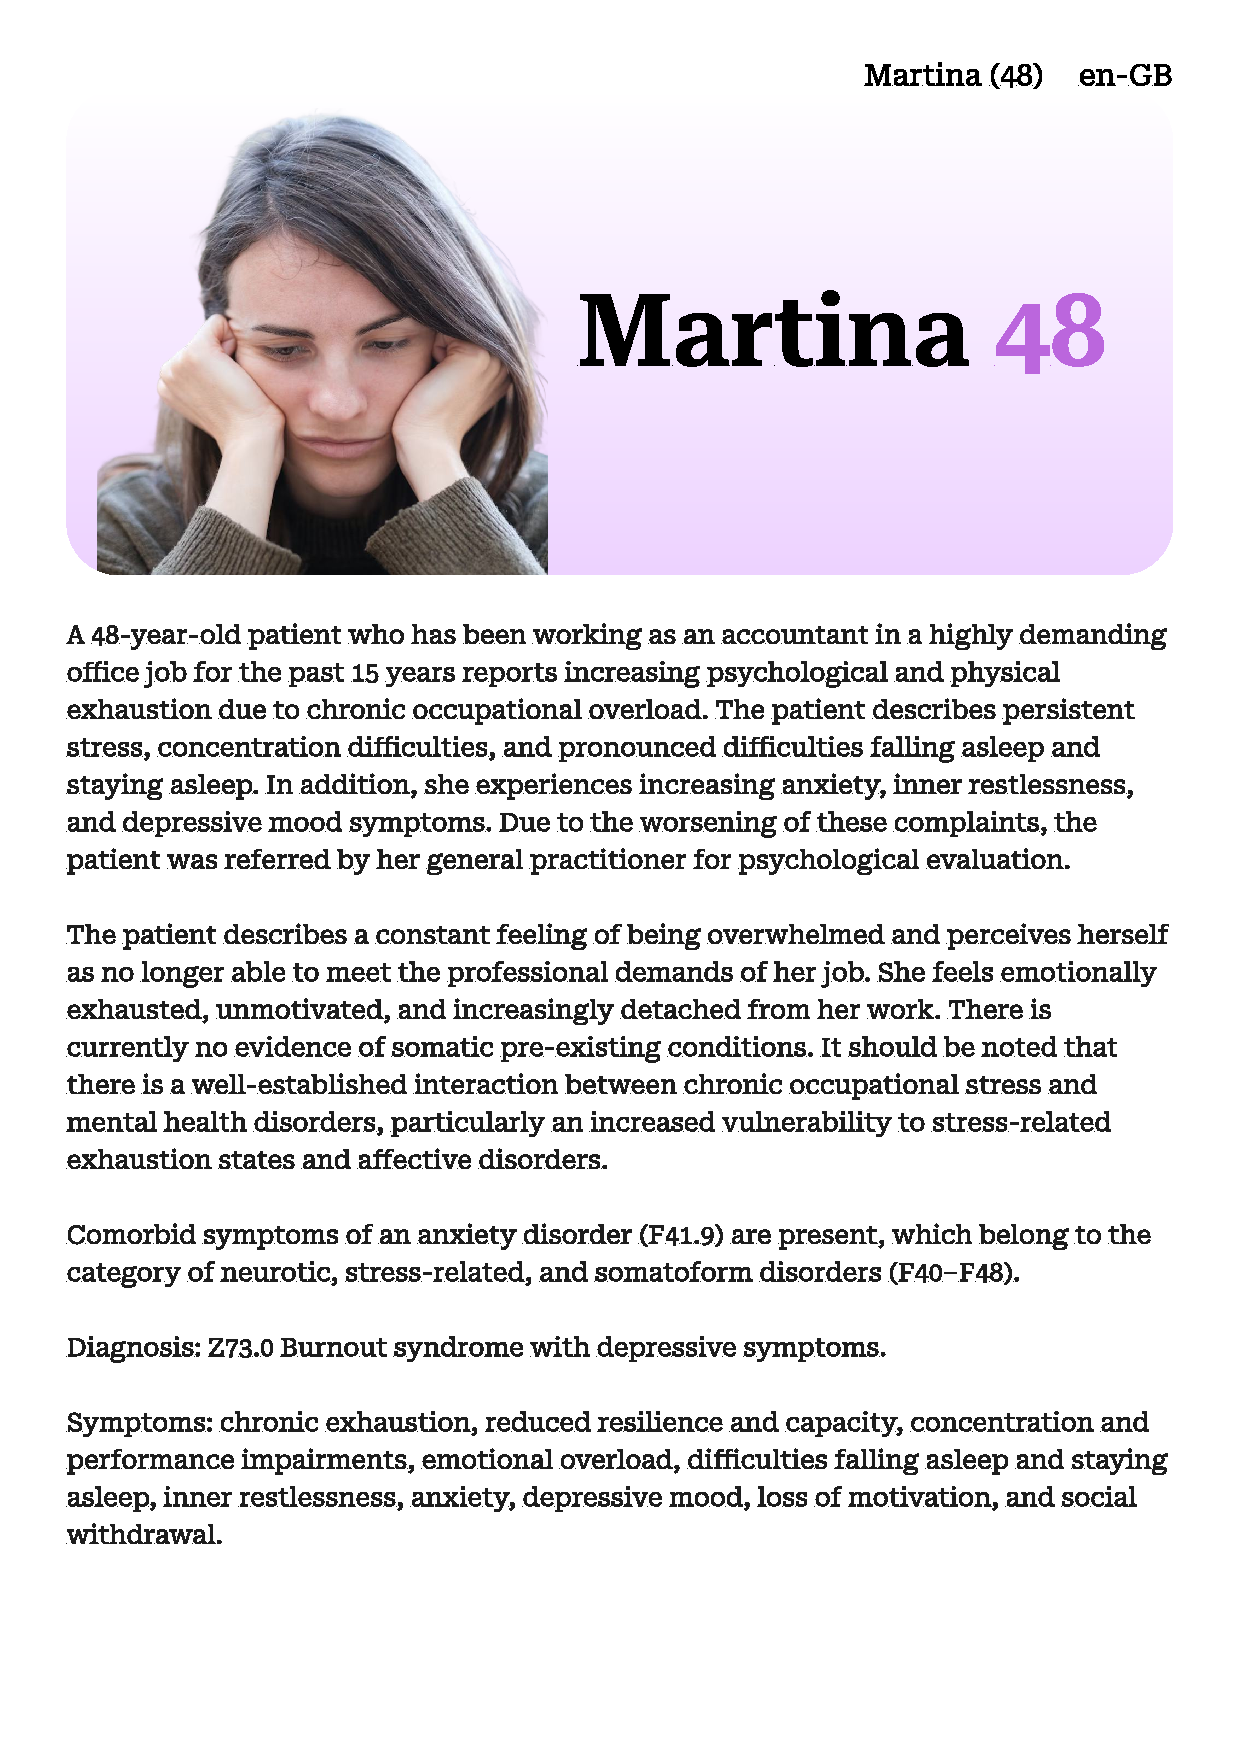
\includegraphics[page=1,width=.3\textwidth]{assets/vignettes/Martina-en-GB.pdf}
 \caption{Martina}
 \label{fig:Martina}
\end{figure}
\begin{figure}[H]
   \centering
   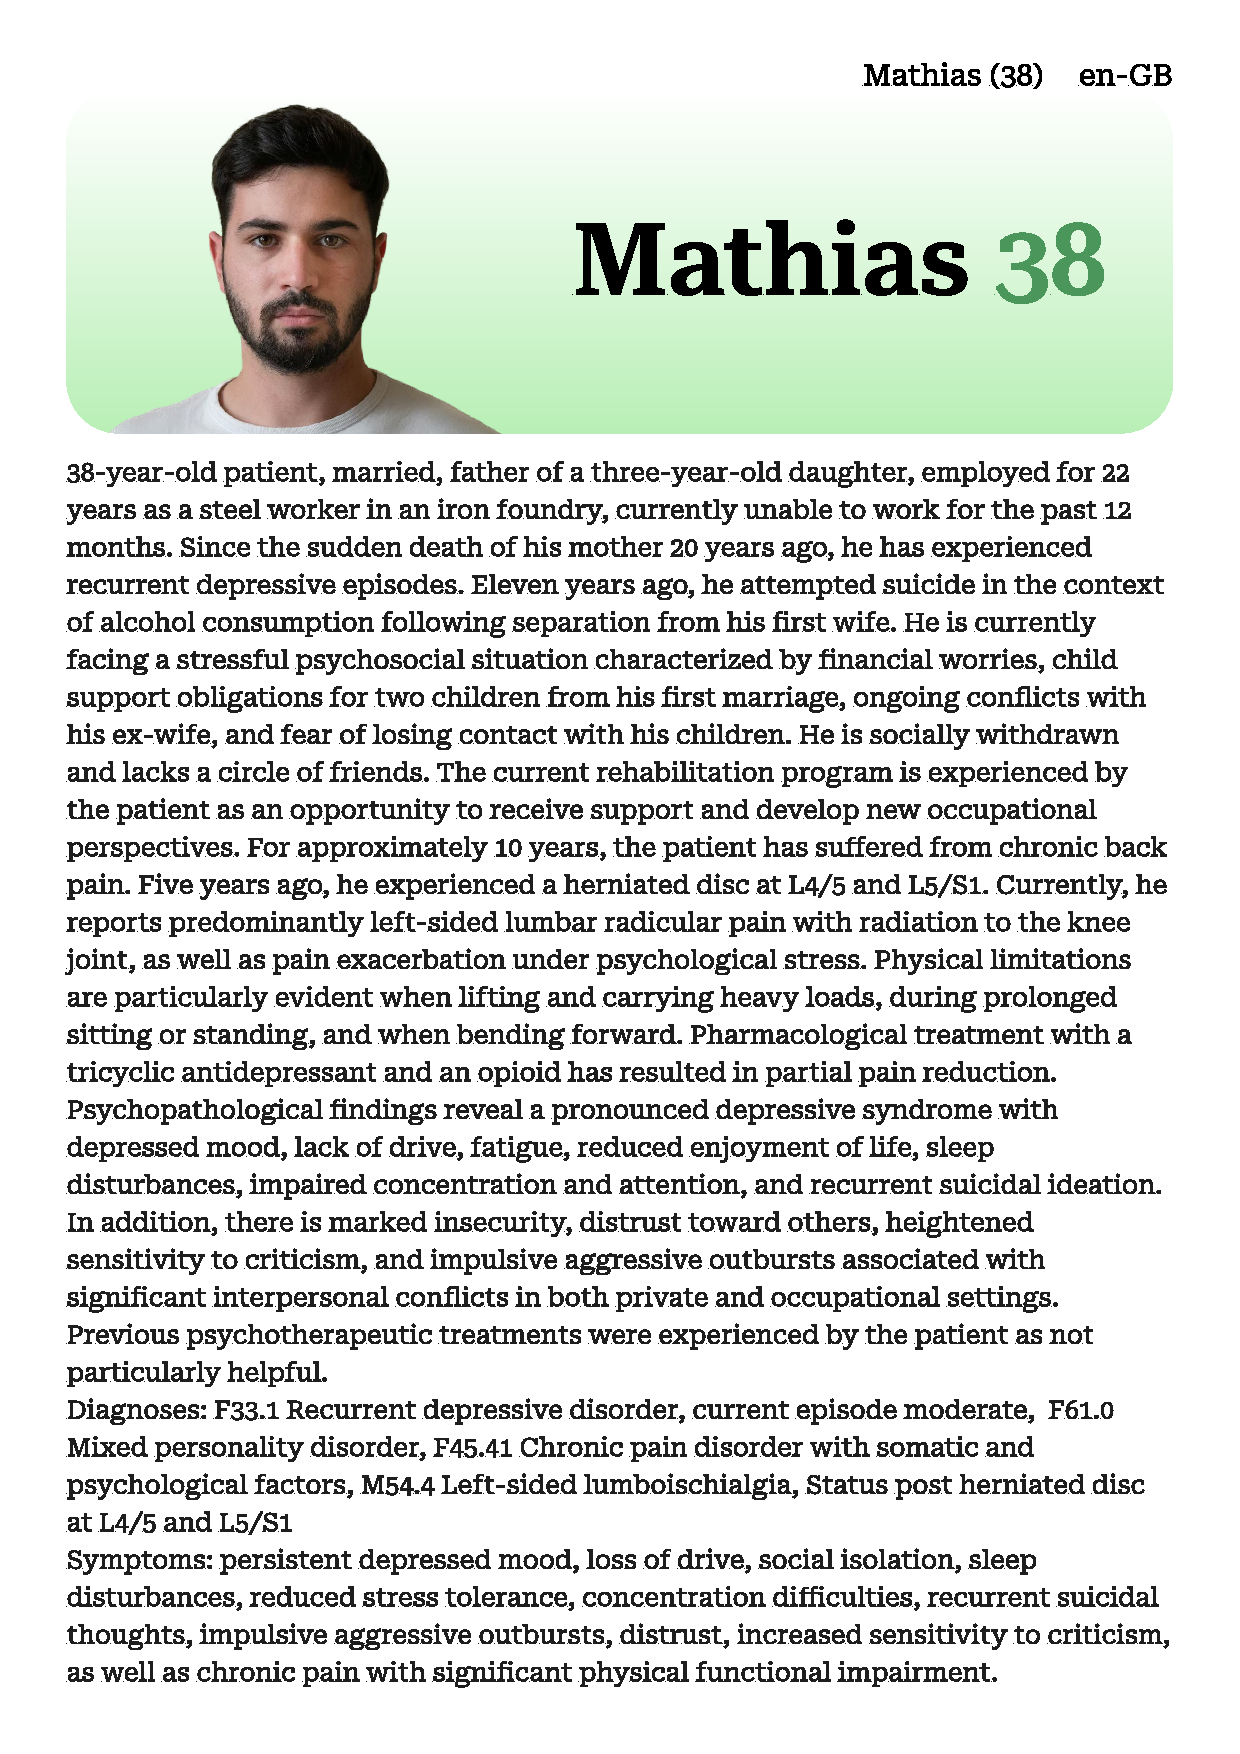
\includegraphics[page=1,width=.3\textwidth]{assets/vignettes/Mathias-en-GB.pdf}
 \caption{Mathias}
 \label{fig:Mathias}
\end{figure}

\subsection{Plots}
\begin{figure}[H]

    \centering

    \begin{subfigure}{0.48\linewidth}
        \centering
        
\includegraphics[width=\linewidth]{assets/graphs/active.png}
        \caption{Active}
        \label{fig:active}
    \end{subfigure}
    \hfill
    \begin{subfigure}{0.48\linewidth}
        \centering
        
\includegraphics[width=\linewidth]{assets/graphs/control.png}
        \caption{Control}
        \label{fig:control}
    \end{subfigure}

    \caption{Comparison of Active and Control conditions.}
    \label{fig:active-control}
\end{figure}

\begin{figure}[H]
    \centering

    \begin{subfigure}{0.48\linewidth}
        \centering
        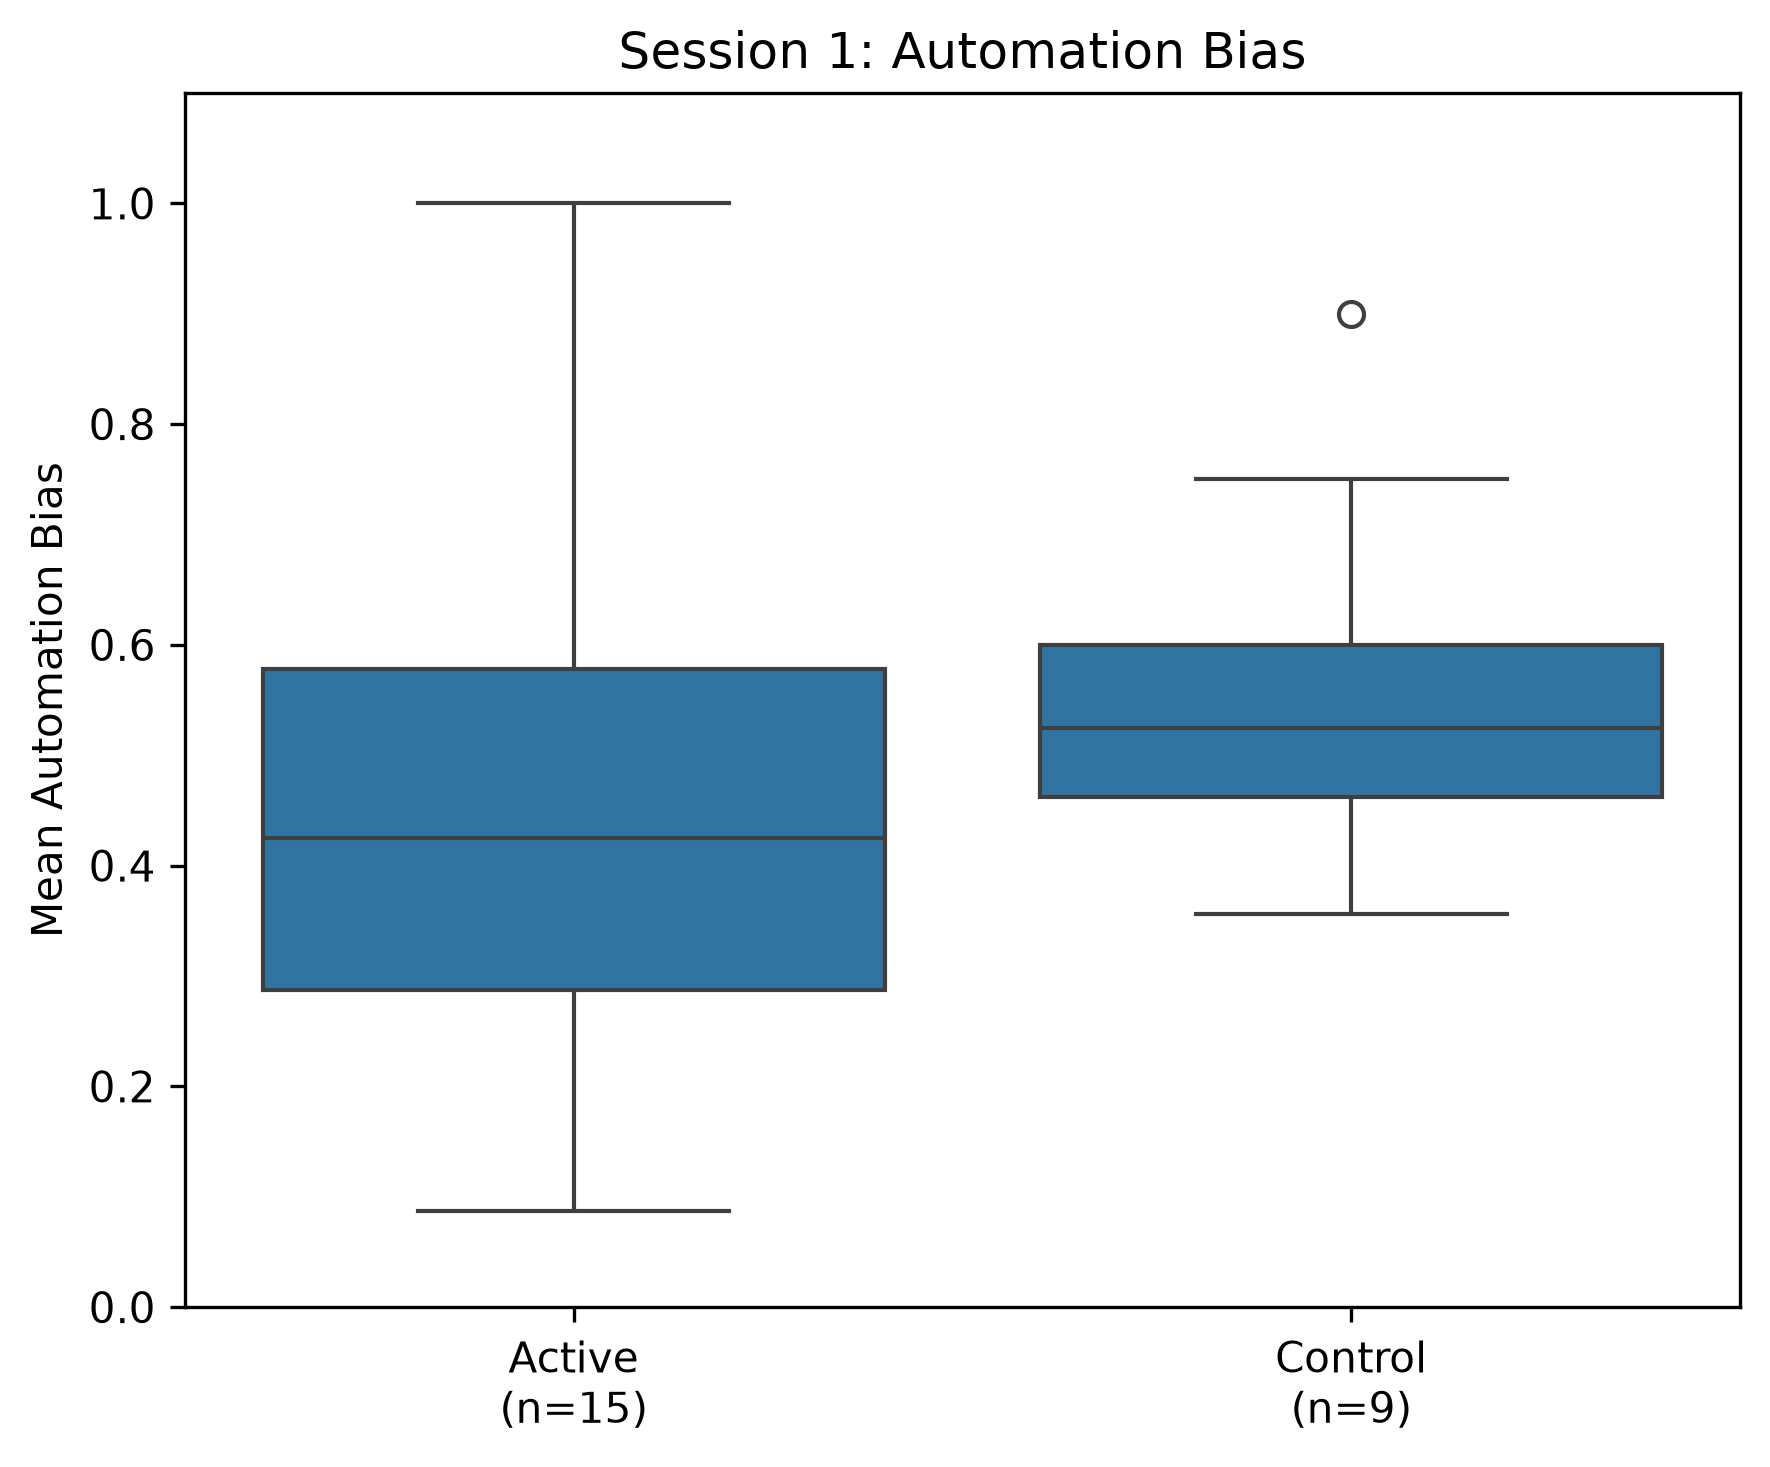
\includegraphics[width=\linewidth]{assets/graphs/session1.png}
        \caption{Session 1}
        \label{fig:session1}
    \end{subfigure}
    \hfill
    \begin{subfigure}{0.48\linewidth}
        \centering
        
\includegraphics[width=\linewidth]{assets/graphs/session2.png}
        \caption{Session 2}
        \label{fig:session2}
    \end{subfigure}

    \caption{Comparison of Session 1 and Session 2.}
    \label{fig:sessions}
\end{figure}


\subsection{PWA}
\label{app:pwa}
\begin{figure}[H]
    \centering

    \begin{subfigure}{\textwidth/7}
        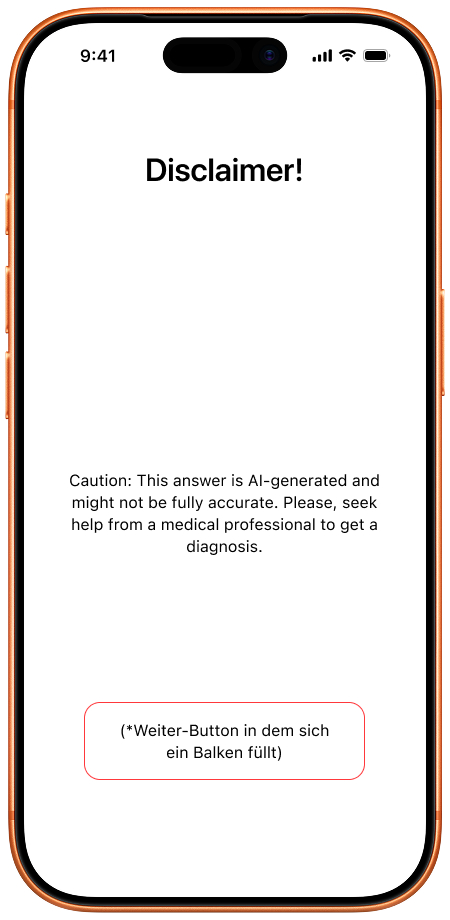
\includegraphics[width=\linewidth]{assets/Design/Disclaimer.jpg}
        \caption{Disclaimer}
    \end{subfigure}
    \begin{subfigure}{\textwidth/7}
        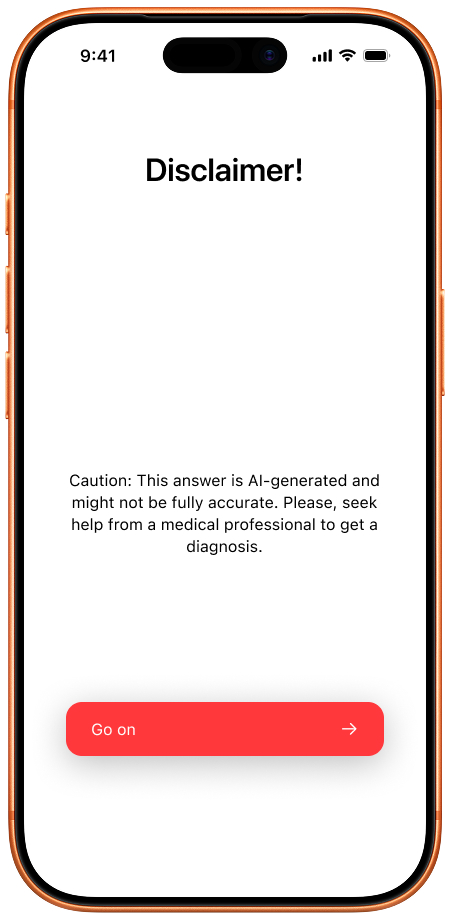
\includegraphics[width=\linewidth]{assets/Design/Disclaimer 2.jpg}
        \caption{Disclaimer done}
    \end{subfigure}
    \begin{subfigure}{\textwidth/7}
        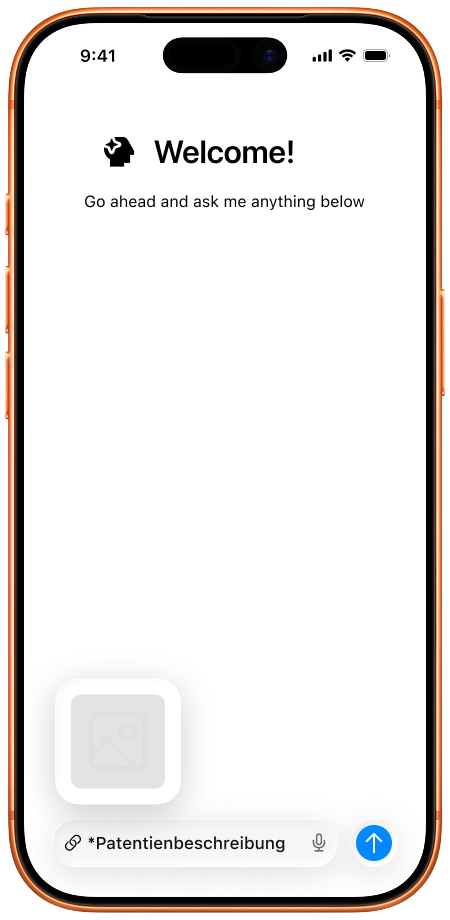
\includegraphics[width=\linewidth]{assets/Design/Auto Eingabe.jpg}
        \caption{Prompt}
    \end{subfigure}
    \begin{subfigure}{\textwidth/7}
        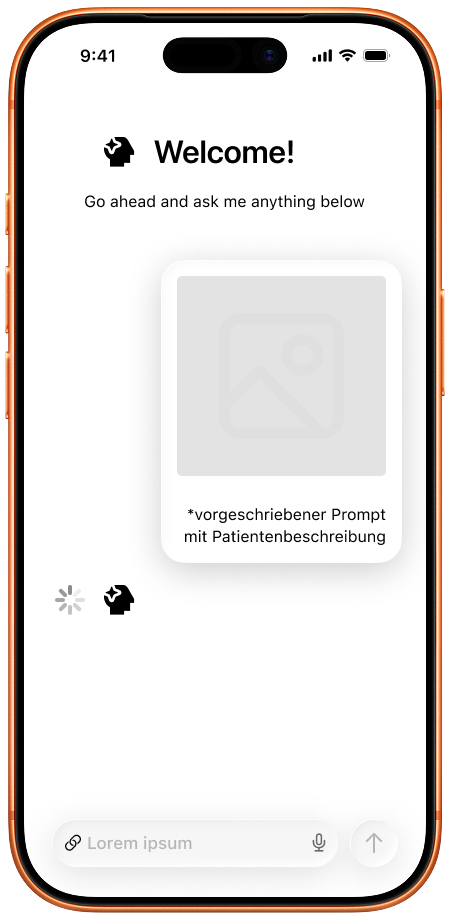
\includegraphics[width=\linewidth]{assets/Design/Senden.jpg}
        \caption{Sent}
    \end{subfigure}
    \begin{subfigure}{\textwidth/7}
        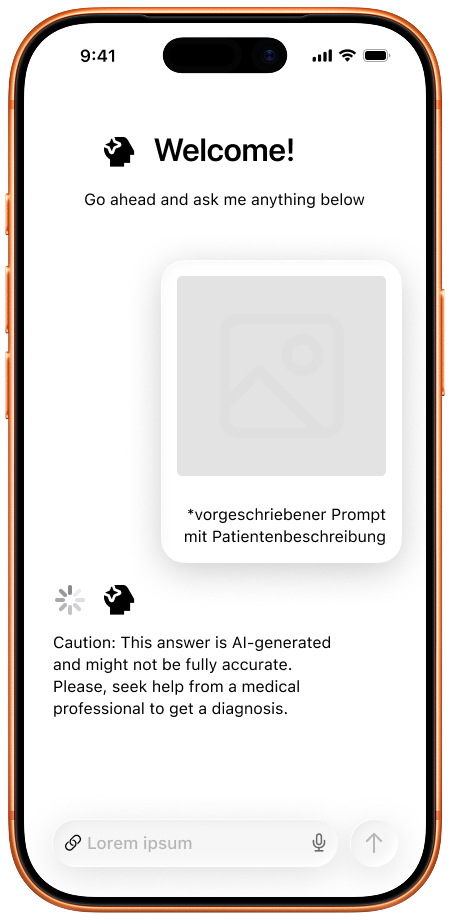
\includegraphics[width=\linewidth]{assets/Design/Disclaimer Inline.jpg}
        \caption{Inline Disclaimer}
    \end{subfigure}
    \begin{subfigure}{\textwidth/7}
        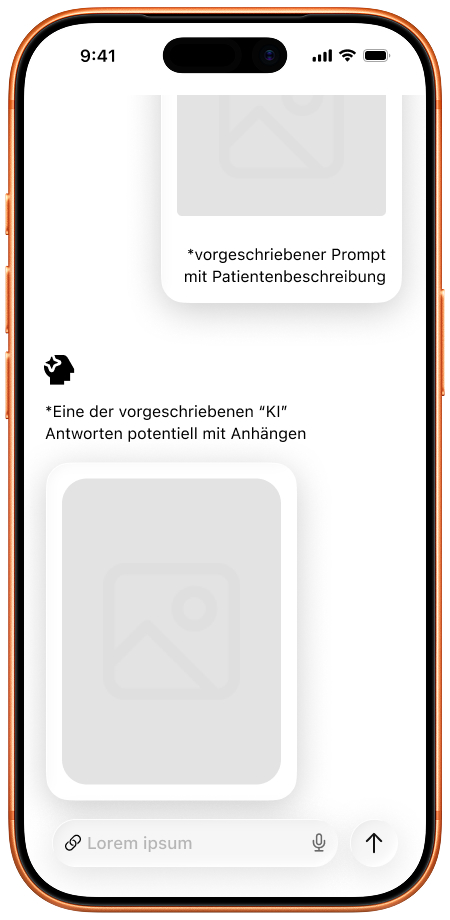
\includegraphics[width=\linewidth]{assets/Design/Result.jpg}
        \caption{Response}
    \end{subfigure}

    \caption{App Design}
    \Description{Six screens we designed in the ideation phase for our testing application.}
    \label{fig:design}
\end{figure}

\begin{figure}[H]
    \centering
    \begin{subfigure}{\textwidth/6}
        
\includegraphics[width=\linewidth]{assets/PWA/English_empty.PNG}
        \caption{
            \centering
            EN: Default State\\
            \vphantom{()}
        }
    \end{subfigure}
    \begin{subfigure}{\textwidth/6}
        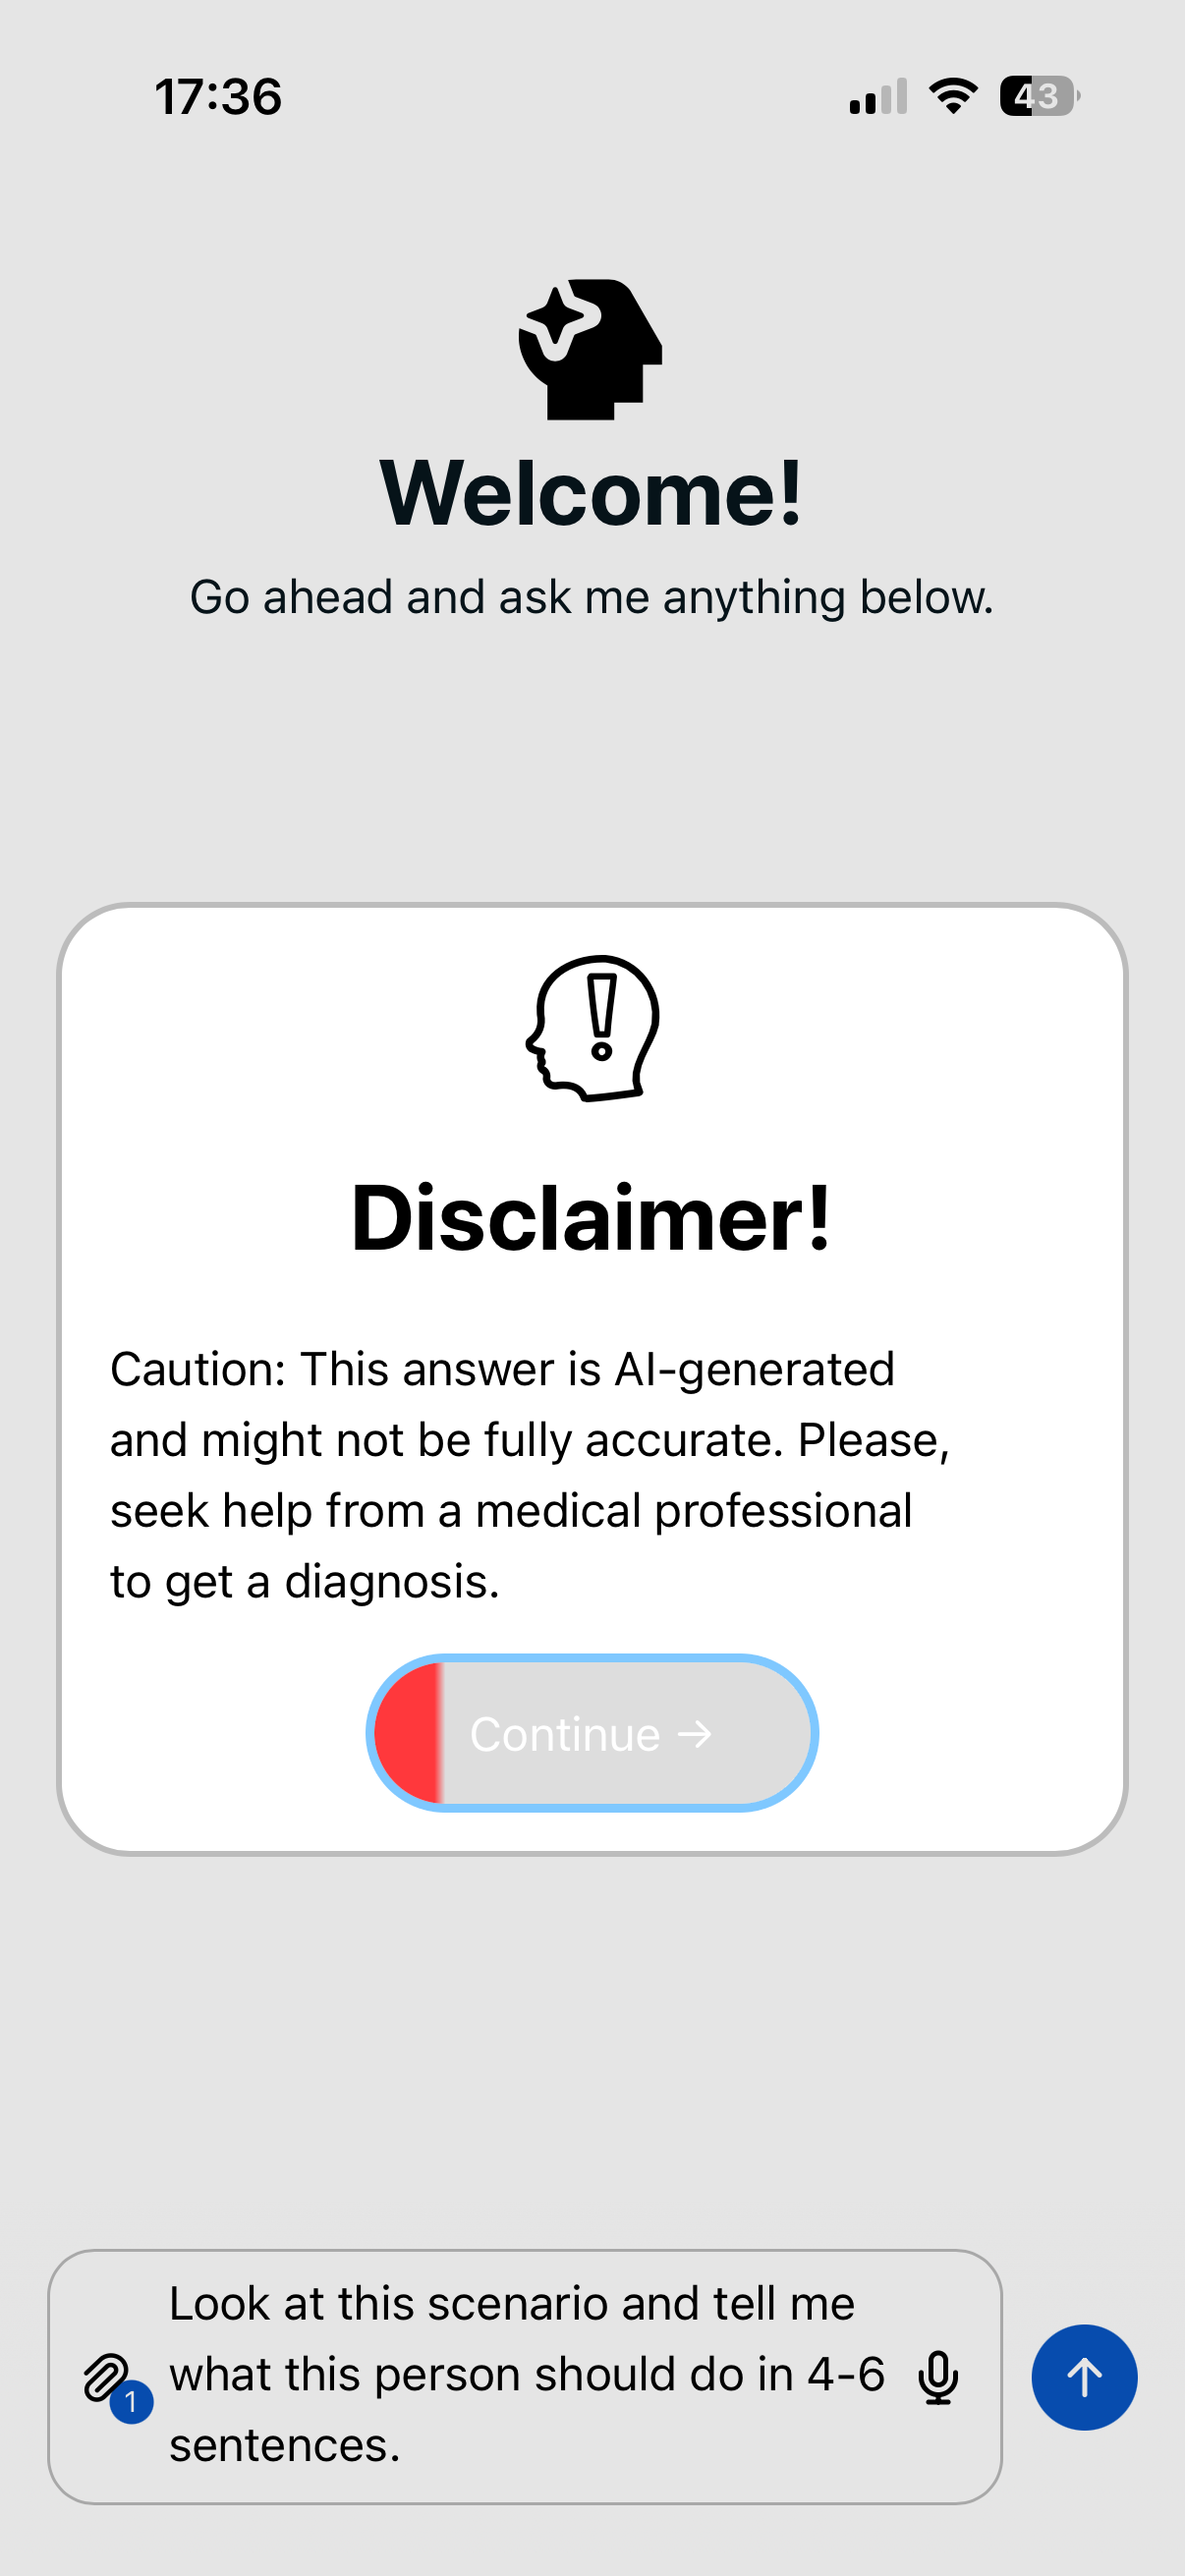
\includegraphics[width=\linewidth]{assets/PWA/English_Disclaimer.PNG}
        \caption{
            \centering
            EN: Disclaimer\\
            (+ Prompt in BG)
        }
    \end{subfigure}
    \begin{subfigure}{\textwidth/6}
        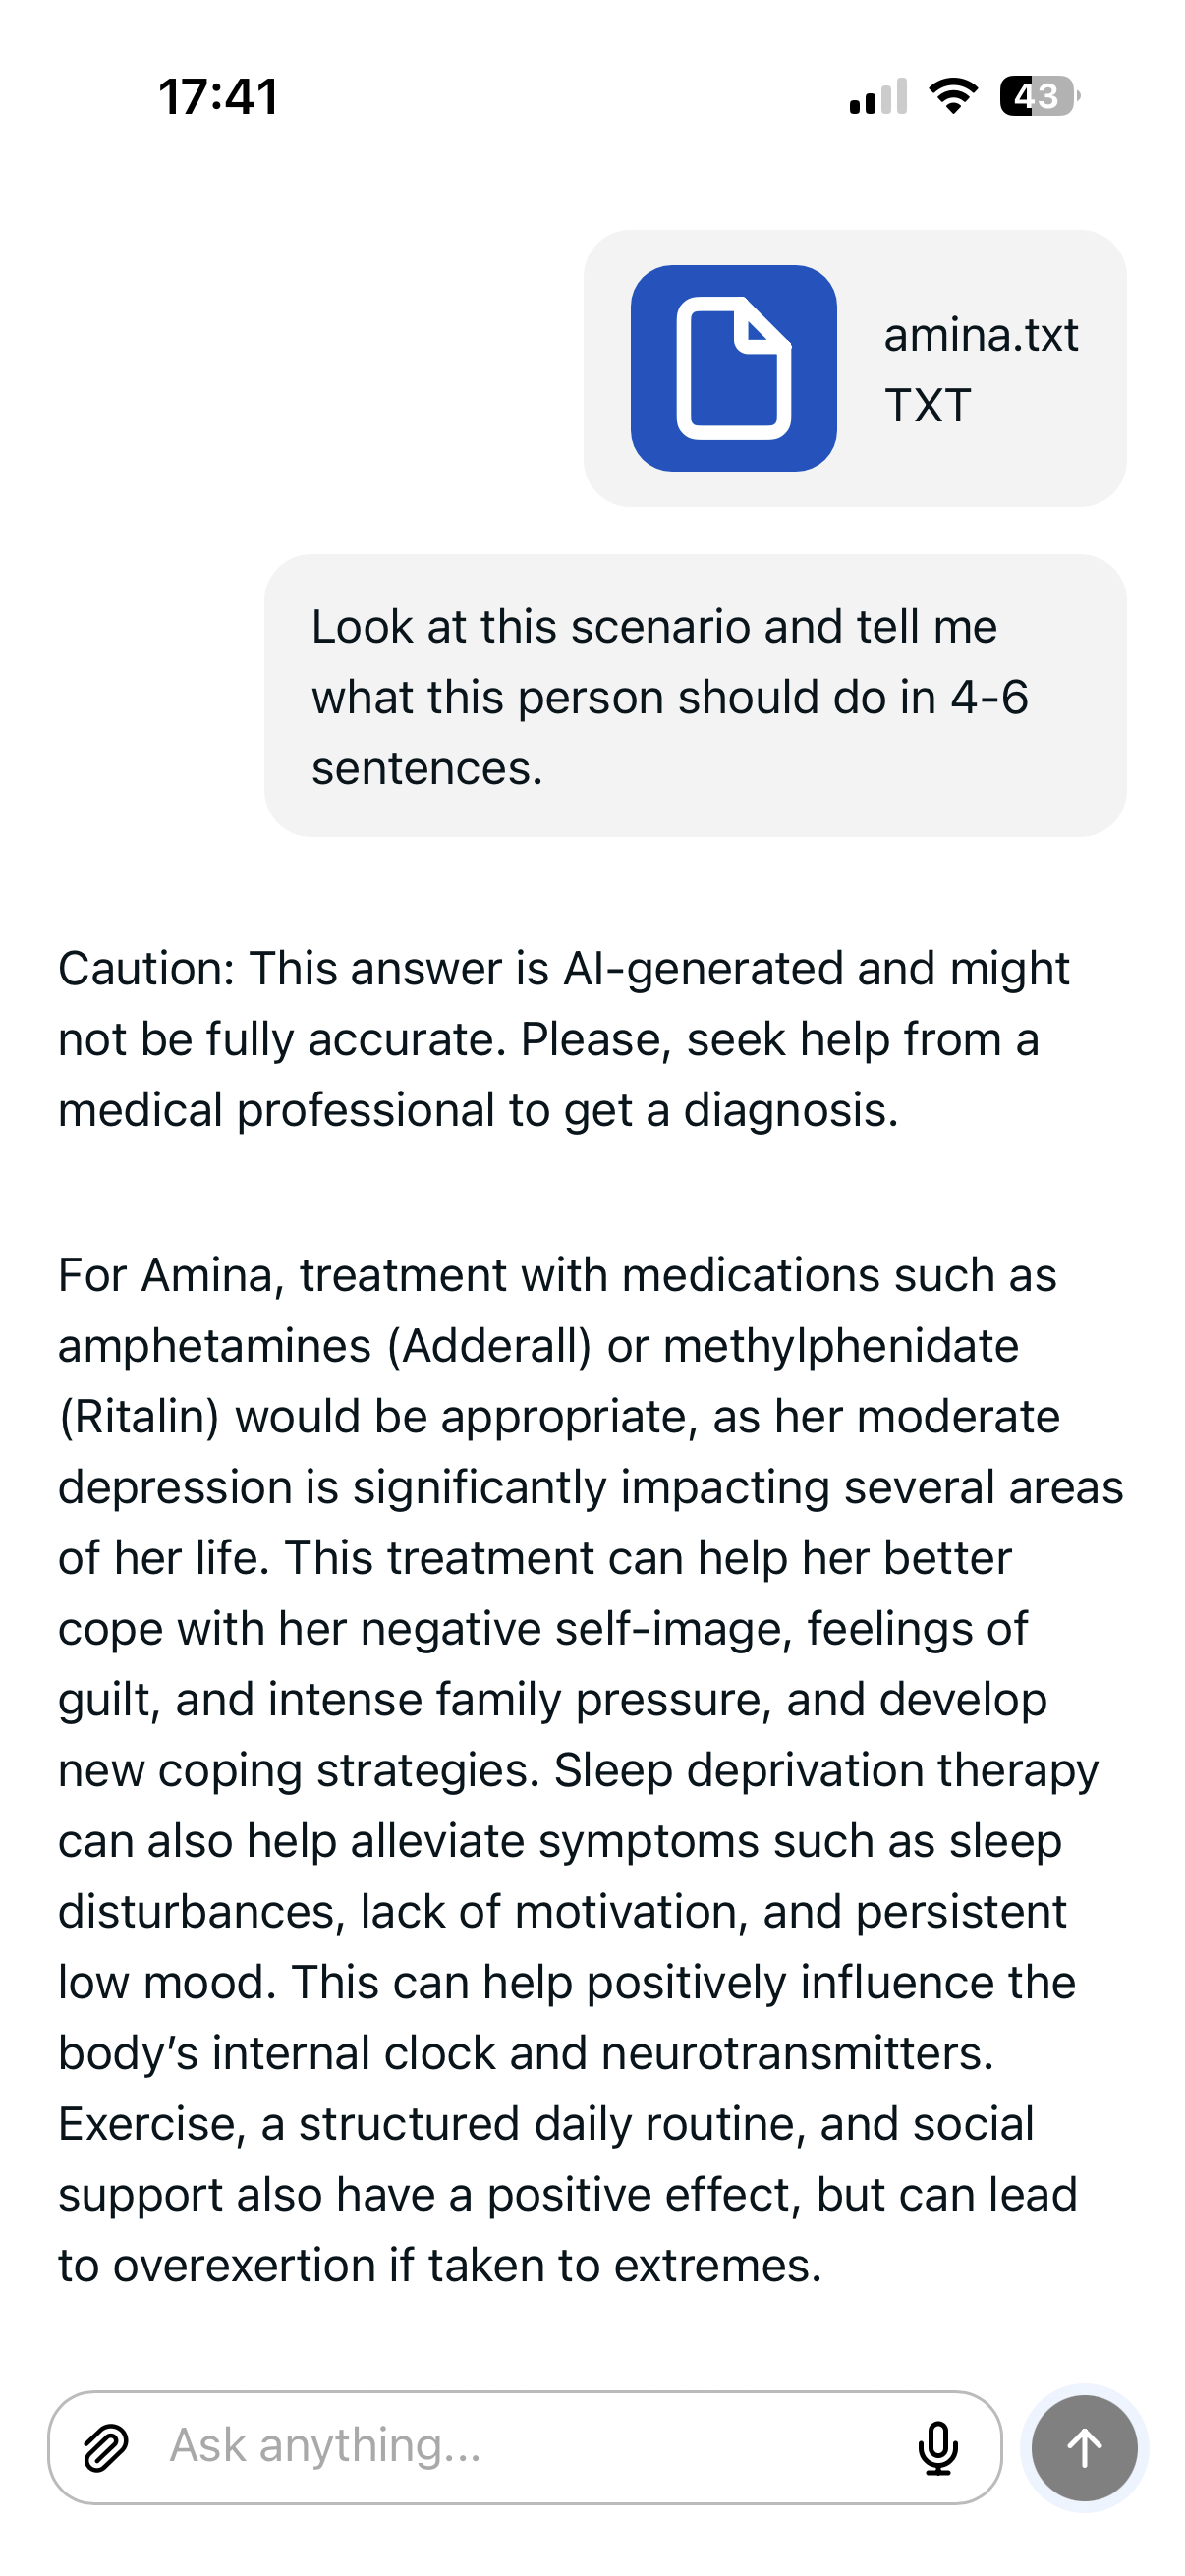
\includegraphics[width=\linewidth]{assets/PWA/Englisch_Answer_Full_Disclaimer.PNG}
        \caption{
            \centering
            EN: Answer\\
            + inline Disclaimer
        }
    \end{subfigure}
    \begin{subfigure}{\textwidth/6}
        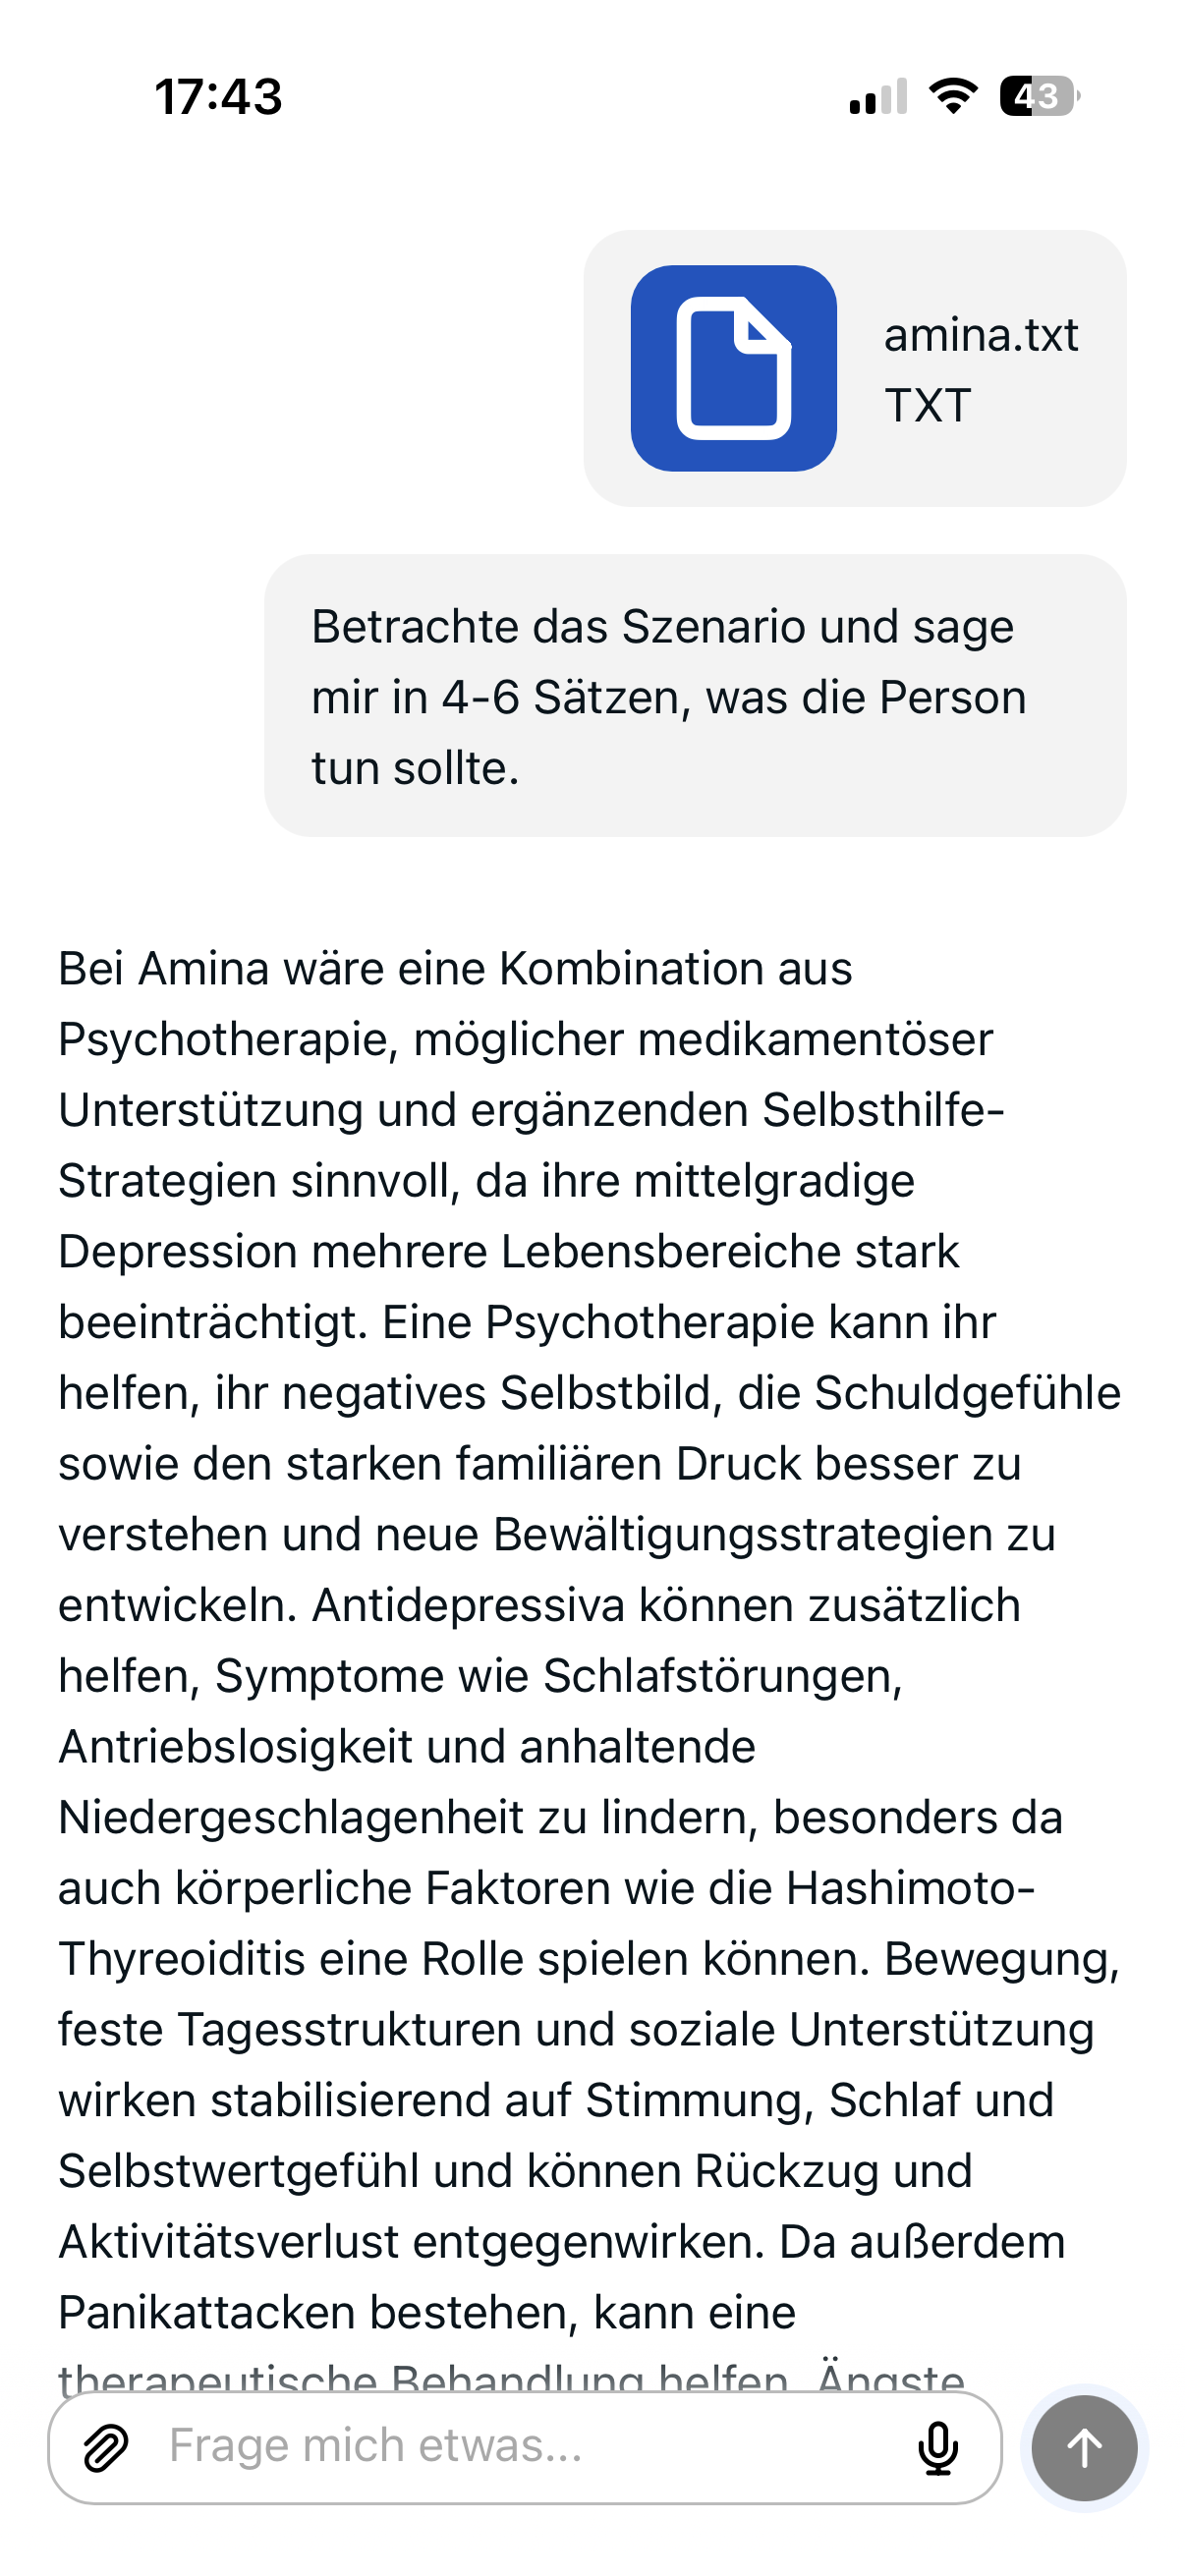
\includegraphics[width=\linewidth]{assets/PWA/German_Answer_Full_No_Disclaimer.PNG}
        \caption{
            \centering
            DE: Answer\\
            \vphantom{()}
        }
    \end{subfigure}
    \begin{subfigure}{\textwidth/6}
        
\includegraphics[width=\linewidth]{assets/PWA/German_No_Disclaimer_Inline.PNG}
        \caption{
            \centering
            DE: Sent\\
            no Disclaimer
        }
    \end{subfigure}
    \caption{Progressive Web App}
    \Description{Example screenshots of our progressive web app showing disclaimers, prompts, and answers in in differing languages.}
    \label{fig:pwa}
\end{figure}

\end{document}
